\section{Introduction}

Several branches of Earth Sciences have demonstrated the importance of spatial resolution on a microscopic scale. For example, geochemistry and
geochronology applications have benefited from point-wise analyses
and compositional maps, allowing significant advances in the understanding of
igneous, metamorphic and sedimentary processes \citep{Verberne2020, Barnes2019,
Davidson2007}. Classical paleomagnetic techniques, on the other hand, consist
of analyzing bulk samples, where the magnetic signal of a single specimen is
the result of the sum of moments of a large assembly of ferromagnetic grains
\citep{Dunlop1997}. Typically, a standard paleomagnetic sample of
approximately \qty{10}{\cm\cubed} would contain hundreds of thousands
to millions of magnetic particles with sizes varying from magnetically stable
single-domain (SD) and vortex state grains (also called pseudo-single domain,
PSD) with sizes below \qty{1}{\um}, to large ($\gg \qty{1}{\um}$) grains with
multi-domain (MD) magnetic structures, which are less stable magnetic recorders
\citep{Berndt2016}. These large MD grains usually conceal the signal of the SD
and PSD grains, and techniques of step-wise thermal and magnetic treatments are
needed to unveil this more stable and reliable magnetic record
\citep{Tauxe2018}. Recently, magnetic microscopy techniques opened the
possibility of obtaining magnetic field maps at the micro-scale and recovering the
magnetization of each grain, therefore enabling the separate analysis of stable
and unstable magnetic particles \citep{DeGroot2018, Lima2014, Weiss2007,
DeGroot2014}.

In order to apply magnetic microscopy to paleomagnetic studies, it is necessary
to recover from the magnetic images a large number of individual magnetic
moments, corresponding to at least tens of thousands of stable fine-grained
grains ($< \qty{1}{\um}$), in order to provide statistical significance to the
remanence vector \citep[e.g., ][]{Berndt2016}. Nowadays, with the development of
magnetic microscopy techniques, this task is no longer limited by the
resolution of magnetic microscopes \citep{Fu2020, Weiss2007, DeGroot2018,
Glenn2017, Lima2014}, but essentially by the intrinsic problem presented by the
ambiguity in the inversion of potential field data \citep{Barbosa2011,
DeGroot2021, Oliveira2015Estimation}, and ultimately by the lack of a fast and
automated way to recover such a large number of individual magnetic moments
from a set of magnetic images \citep{CortesOrtuno2022, Lima2013, Lima2009}. A
solution to the non-uniqueness of magnetic moment inversion is to add
independent prior information, such as the position of the ferromagnetic
particles \citep{Fabian2019}. This can be obtained, for example, from X-ray
computed tomography \citep[microCT; ][]{Fabian2019, DeGroot2021, DeGroot2018}.
Nonetheless, the standard microCT techniques do not provide adequate resolution
to resolve the finer and more stable magnetic grains \citep{CortesOrtuno2022,
DeGroot2021}, whereas other more sophisticated techniques such as ptychographic
X-ray tomography \citep[e.g., ][]{Maldanis2020} are not readily available and
too time-consuming to be routinely used in paleomagnetic studies.

Another route to be explored in the inversion of magnetic microscopy images is
to obtain all the information, i.e. the magnetic moment and the position of the
sources, from the magnetic data itself \citep[e.g., ][]{Fu2020}. For that, we can
explore the techniques developed in exploration geophysics, in spite of the
differences between aeromagnetic surveys and magnetic microscopy
\citep{Lima2013}. Magnetic microscopy images commonly show the combined signal
of multiple magnetic particles and can vary greatly in wavelength, strength,
and spatial separation, depending on the natural remanent magnetization (NRM) and location of each particle. We
usually assume that the signal measured by the magnetic microscope is the
vertical component of the magnetic induction vector ($b_z$), the measurements
are performed on a regular grid with evenly spaced grid points and at a
constant height, and the data are contaminated with pseudorandom Gaussian noise and
long-wavelength noise (akin to a regional signal in aeromagnetic data). Here,
we provide a methodological routine to retrieve the individual magnetic moment
of ferromagnetic grains in magnetic microscopy images following the approach
devised by \citet{Oliveira2015Estimation} for the interpretation of
aeromagnetic anomalies. The method we propose allows one to quickly and
semi-automatically estimate the individual magnetic moment vector of the stable
magnetic carriers, making use of only the magnetic images themselves and an
assumption of approximately dipolar sources. If used on a large scale, the
method provides the means to scan large areas of the rock sample, attaining
potentially the number of magnetic moments necessary for paleomagnetic studies.


%%%%%%%%%%%%%%%%%%%%%%%%%%%%%%%%%%%%%%%%%%%%%%%%%%%%%%%%%%%%%%%%%%%%%%%%%%%%%%%
\section{Methodology}

We will achieve the goal of estimating the dipole moment of several individual
grains per image in a semi-automatic fashion by dividing the task into three
parts that can be performed independently:

\begin{enumerate}
\item \textbf{Source detection and separation:} Identify and spatially isolate
  the magnetic field caused by each source. We will do this through a
  combination of classic potential field data processing (\textit{total
  gradient amplitude}) and image processing (histogram stretching and
  equalization) and segmentation methods (watershed segmentation).
\item \textbf{Position estimation}: Estimate the 3D position of a magnetic
  particle based on the magnetic field measurements and the assumption of a
  dipolar source. This can be achieved by applying the Euler Deconvolution
  method to the data segment identified in step 1.
\item \textbf{Magnetic moment inversion:} Estimate the 3-component dipole
  moment vector by inverting the magnetic field data using the position
  obtained from Euler Deconvolution as a constraint and the assumption of a
  dipolar source. This leads to a linear inverse problem that is stable and
  computationally efficient, particularly since the inversion is performed
  separately for each data segment identified in step 1.
\end{enumerate}

In the sections below, we describe the methodology used in each step of our
proposed workflow.

\subsection{Automatic source detection and separation}

Our first task is to automatically identify the signal of individual particles
and spatially segregate the data into windows, each containing the signal of a
single particle. We implemented the following workflow to achieve this:

\begin{enumerate}
\item Calculate the \textit{total gradient amplitude} (TGA), also known as the 3D analytic signal \citep{Roest1992Magnetic}, of the observed vertical   component of the magnetic field. The TGA is entirely positive and tends to be more concentrated on top of the magnetic field sources than the observed magnetic field. The derivative calculation also acts as a high-pass filter, removing long-wavelength noise from the data.
\item Apply a contrast stretching method to re-scale the TGA to a new range   defined by the lower and upper percentiles of the data in order to highlight the weaker signals, either coming from small or from deep-seated particles.
\item Use the Laplacian of Gaussian (LoG) method \citep{VanderWalt2014} on the   re-scaled TGA data to estimate the position and size of data windows containing the signal of each particle.
\end{enumerate}

The total gradient amplitude (TGA) was devised as a filter that can be applied
to aeromagnetic data to reduce the signal's dependence on the direction of
magnetization of the source and that concentrates the signal above the sources
\citep{Roest1992Magnetic, Nabighian2005}. The TGA is defined as the norm of the
gradient vector of a scalar field $f(x, y, z)$

\begin{equation}
\|\vec{\mathbf{\nabla}}f(x, y, z)\|  =
\sqrt{(\partial_x f)^2 + (\partial_y f)^2 + (\partial_z f)^2}
\ ,
\end{equation}

\noindent
in which $\partial_x f$ is the partial derivative of $f$ with respect to $x$
and likewise for the $y$ and $z$ directions. The partial derivatives are best
approximated using a second-order accurate central finite-difference scheme

\begin{equation}
\partial_x f(x, y, z) \approx
\dfrac{f(x + \Delta x, y, z) - f(x - \Delta x, y, z)}{2 \Delta x}
\ ,
\end{equation}

\noindent
and likewise for the $y$ and $z$ directions, in which $\Delta x$ is the grid
spacing (assumed to be equal in the $x$ and $y$ directions). For the $z$
component, $\Delta z = \Delta x$ and $f(x, y, z + \Delta z)$ and
$f(x, y, z - \Delta z)$ are calculated by upward and downward continuation,
respectively, performed in the wavenumber domain. The 2D maps of the $x$, $y$,
and $z$ derivatives will also be used in the Euler Deconvolution step described
below, which is known to be highly sensitive to noise in the derivatives
\citep{Saleh2012Applying}. This is why we prefer the finite-differences based
derivatives, which are less prone to amplifying short-wavelength noise than
those calculated in the wavenumber domain through the Fast Fourier Transform
(FFT).

Once we have obtained a TGA image, we apply a contrast stretching method to
re-scale the TGA values in order to highlight the weaker signals present in the
image. This is a necessary step to make sure that the blob detection algorithm
is able to identify particles causing both weak and strong signals. The
following contrast stretching operation is performed per pixel of the TGA image

\begin{equation}
\text{TGA}_{rescaled} =
2\left(\dfrac{\text{TGA} - v_{min}}{v_{max} - v_{min}}\right) - 1
\ ,
\end{equation}

\noindent
in which $v_{min}$ and $v_{max}$ are the upper and lower bounds of TGA values
that will be stretched to the range $[0, 1]$. By experimentation, we found
that values of $v_{min} = 1^\text{st}$ and $v_{max} = 99^\text{th}$
percentiles of the TGA range work well on real magnetic microscopy datasets.

The re-scaled TGA image is then used as input for a Laplacian of Gaussian (LoG)
blob detection algorithm \citep{Kong2013}. This method is able to identify the
location and size of multiple windows in the image containing ``blobs''. In our
case, the blobs are the re-scaled TGA field of each particle and the LoG method
detects the local TGA maxima. The LoG method is particularly well suited for
the detection of bright blobs on a dark background at the expense of a longer
computation time \citep{Han2016}. For the image sizes routinely found in
magnetic microscopy, the computation is fast and only needs to be performed
once per image.

\subsection{Euler Deconvolution}

Once the locations and sizes of the windows containing the isolated signals of
each particle are determined, we can apply the Euler Deconvolution (ED)
estimate of the $x$, $y$, and $z$ positions of the center of the particles
under a dipolar approximation. This technique was first proposed by
\citet{Thompson1982} under the name EULDPH and later extended to three
dimensions and renamed ``Euler Deconvolution'' by \citet{Reid1990}. ED is
traditionally performed on a set of moving windows that scan the entire
dataset, producing a large scatter of position estimates, most of which are
spurious \citep{Silva20033D}. This is only done because it is impractical to
segment an aeromagnetic dataset into individual anomalies. Fortunately,
magnetic microscopy images often contain fewer elongated features (e.g., dikes and
suture zones) and regional signals (e.g., Curie depth variations) that are
difficult to separate. This makes it possible for us to produce isolated
signals for each magnetic particle through the source detection step described
above. Since each data window contains only the signal of a single particle, we
are able to apply ED and generate only a single position estimate per particle.

\begin{figure}[tb]
\centering
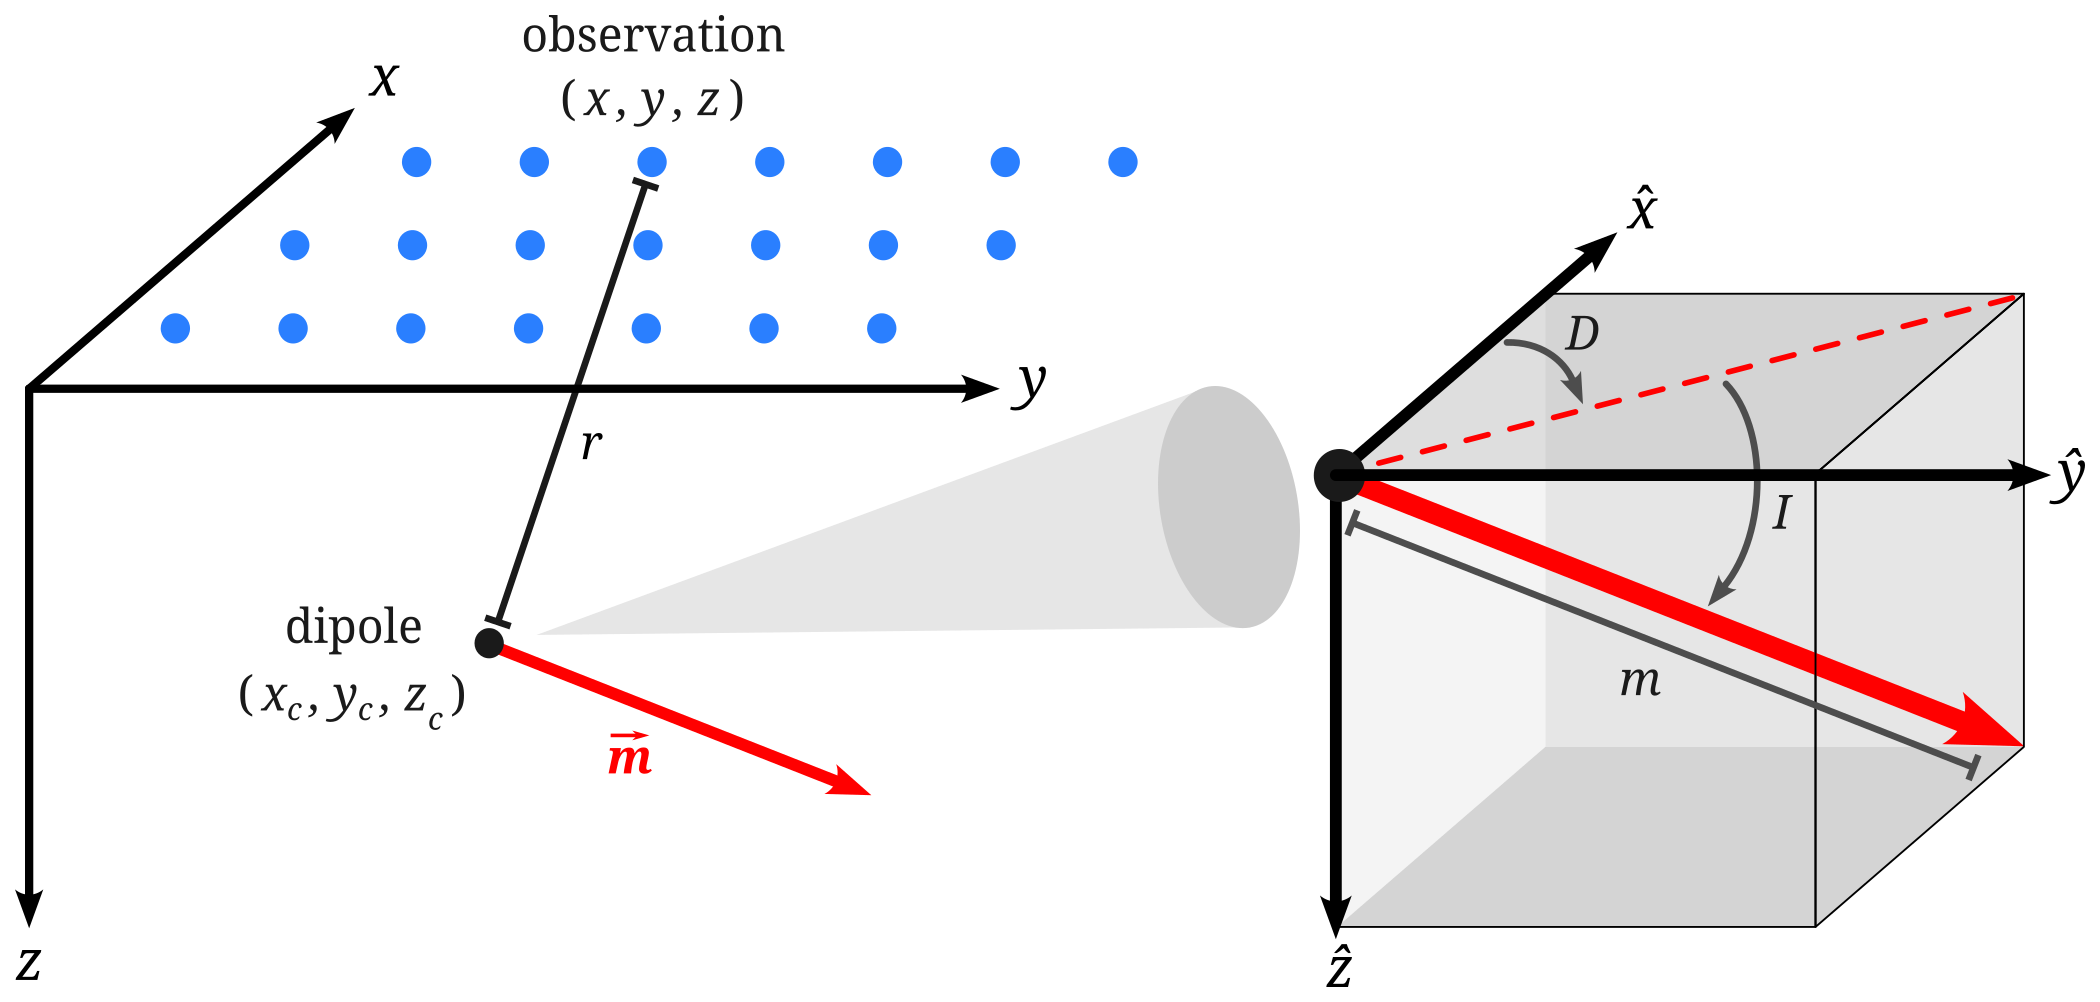
\includegraphics[width=\linewidth]{figures/coordinate-system-sketch.png}
\caption{
Schematic representation of the coordinates systems and modelling elements.
The left panel shows the $x, y, z$ right-handed coordinate system with $z$
pointing upward and away from the sample. The top surface of the sample defines
the $z=0$ surface. A dipole with dipole moment vector $\mathbf{\vec{m}}$ is
also shown at coordinates $(x_c, y_c, z_c)$. The observation points are located
at regular intervals on an $x-y$ plane at a positive $z$ separation from the
sample surface. The right panel zooms in on the dipole and shows the dipole
moment vector expressed in terms of inclination ($I$, positive downwards),
declination ($D$, angle with the $\hat{y}$ direction), and moment magnitude $m
= \|\mathbf{m}\|$.
}
\label{fig_coordinate_systems}
\end{figure}

Euler Deconvolution is formulated as a least-squares inversion of Euler's
homogeneity equation

\begin{equation}
\label{eq_euler_homogeneity}
(x - x_c)\partial_x f
+ (y - y_c)\partial_y f
+ (z - z_c)\partial_z f
= (b - f)\eta
\ ,
\end{equation}

\noindent
in which $(x_c, y_c, z_c)$ are the coordinates of the magnetic field source (Figure~\ref{fig_coordinate_systems}), $b$ is the base level representing a constant shift in the signal, and $\eta$ is the structural index corresponding to the nature of the source \citep{Reid1990}. This equation holds true for simple geometric sources, like spheres, dipoles, and vertical cylinders. Here, we assume that the magnetic particles are small enough and the sensor is far enough away that the sources can be represented by dipoles, yielding an $\eta=3$.

The inversion is performed by rearranging Equation~\ref{eq_euler_homogeneity} into a pseudo-parametric model with parameters $x_c$, $y_c$, $z_c$, and $b$

\begin{equation}
x_c \partial_x f + y_c \partial_x f + z_c \partial_x f + \eta b
=
x \partial_x f + y \partial_y f + z \partial_z f + \eta f
\ .
\end{equation}

Given a set of $N$ observations of the magnetic field as the harmonic function $f$ and its spatial derivatives, we can form the $N \times 4$ system of equations

\begin{equation}
\begin{bmatrix}
  {\partial_x f}_1 & {\partial_y f}_1 & {\partial_z f}_1 & \eta \\
  {\partial_x f}_2 & {\partial_y f}_2 & {\partial_z f}_2 & \eta \\
  \vdots & \vdots & \vdots & \vdots \\
  {\partial_x f}_N & {\partial_y f}_N & {\partial_z f}_N & \eta
\end{bmatrix}
\begin{bmatrix}
  x_c \\ y_c \\ z_c \\ b
\end{bmatrix}
=
\begin{bmatrix}
  x_1 {\partial_x f}_1 + y_1 {\partial_y f}_1 + z_1 {\partial_z f}_1 + \eta f_1 \\
  x_2 {\partial_x f}_2 + y_2 {\partial_y f}_2 + z_2 {\partial_z f}_2 + \eta f_2 \\
  \vdots \\
  x_N {\partial_x f}_N + y_N {\partial_y f}_N + z_N {\partial_z f}_N + \eta f_N \\
\end{bmatrix}
\ .
\end{equation}

In matrix notation, this linear system can be written as

\begin{equation}
\label{eq_euler_forward}
\mathbf{G} \mathbf{p} = \mathbf{h} \ .
\end{equation}

We can arrive at a solution to Equation~\ref{eq_euler_forward} by assuming that the three spatial derivatives of $f$ have negligible error and minimizing the misfit $\phi(\mathbf{p})$ between a pseudo-observation vector $\mathbf{h}^o$ and the predictions $\mathbf{h}$. The least-squares misfit $\phi(\mathbf{p})$ is defined as

\begin{equation}
\label{ZTSuSBbL16}
\phi(\mathbf{p}) = \|\mathbf{h}^o - \mathbf{h}\|^2 = (\mathbf{h}^o - \mathbf{G}\mathbf{p})^T (\mathbf{h}^o - \mathbf{G}\mathbf{p})\ .
\end{equation}

The minimum of $\phi(\mathbf{p})$ is obtained by solving the $4 \times 4$
system of normal equations

\begin{equation}
\mathbf{G}^T \mathbf{G} \mathbf{p} = \mathbf{G}^T \mathbf{h}^o\ .
\end{equation}

The solution vector $\hat{\mathbf{p}}$ provides an estimate of the position
$(x_c, y_c, z_c)$ and base level $b$ for the source located inside of a data
window. Repeating this process for each window produced by the source detection
algorithm will yield the horizontal locations and depths of each magnetic
particle.

\subsection{Magnetic moment inversion}

Once the source position is known and we can assume that it is approximately
spherical or dipolar, we can apply the method developed by
\citet{Oliveira2015Estimation} to estimate the dipole moment vector
$\mathbf{m}$ of the source. We begin by following
\citet{Oliveira2015Estimation} in formulating the magnetic induction vector
$\mathbf{b}$ of a dipole as

\begin{equation}
\label{eq_vector_dipole_field}
\mathbf{b}
=
\begin{bmatrix}
  b_x \\ b_y \\ b_z
\end{bmatrix}
= \dfrac{\mu_0}{4\pi}
\begin{bmatrix}
    \dfrac{\partial^2}{\partial x \partial x} \dfrac{1}{r}
  & \dfrac{\partial^2}{\partial x \partial y} \dfrac{1}{r}
  & \dfrac{\partial^2}{\partial x \partial z} \dfrac{1}{r}
  \\
    \dfrac{\partial^2}{\partial y \partial x} \dfrac{1}{r}
  & \dfrac{\partial^2}{\partial y \partial y} \dfrac{1}{r}
  & \dfrac{\partial^2}{\partial y \partial z} \dfrac{1}{r}
  \\
  \dfrac{\partial^2}{\partial z \partial x} \dfrac{1}{r}
  & \dfrac{\partial^2}{\partial z \partial y} \dfrac{1}{r}
  & \dfrac{\partial^2}{\partial z \partial z} \dfrac{1}{r}
\end{bmatrix}
\begin{bmatrix}
  m_x \\ m_y \\ m_z
\end{bmatrix}
= \dfrac{\mu_0}{4\pi} \mathbf{M}\,\mathbf{m}
\ ,
\end{equation}

\noindent
in which $r = \sqrt{(x - x_c)^2 + (y - y_c)^2 + (z - z_c)^2}$ is the Cartesian distance between the observation point $(x, y, z)$ and the source $(x_c, y_c, z_c)$ and $\mu_0$ is the vacuum magnetic permeability. Most magnetic microscopes provide measurements of only the vertical component $b_z$, which can be isolated from Equation~\ref{eq_vector_dipole_field} as shown in Equation~\ref{eq_dipole_bz}, which is a similar approach to the uniform model proposed by \cite{Weiss2007}.

\begin{equation}
\label{eq_dipole_bz}
b_z
= \dfrac{\mu_0}{4\pi}
\begin{bmatrix}
\dfrac{\partial^2}{\partial z \partial x} \dfrac{1}{r}
& \dfrac{\partial^2}{\partial z \partial y} \dfrac{1}{r}
& \dfrac{\partial^2}{\partial z \partial z} \dfrac{1}{r}
\end{bmatrix}
\begin{bmatrix}
m_x \\ m_y \\ m_z
\end{bmatrix}
= \dfrac{\mu_0}{4\pi} \mathbf{M_z}\,\mathbf{m}
\ .
\end{equation}

The three second-order derivatives in Equation~\ref{eq_dipole_bz} are

\begin{equation}
\begin{aligned}
\dfrac{\partial^2}{\partial z \partial x} \dfrac{1}{r} &=
\dfrac{3(z - z_c)(x - x_c)}{r^5}\ ,
\\
\dfrac{\partial^2}{\partial z \partial y} \dfrac{1}{r} &=
\dfrac{3(z - z_c)(y - y_c)}{r^5}\ ,
\\
\dfrac{\partial^2}{\partial z \partial z} \dfrac{1}{r} &=
\dfrac{3(z - z_c)^2}{r^5} - \dfrac{1}{r^3}\ .
\end{aligned}
\end{equation}

Given a set of $N$ observations of $b_z$ made inside a window containing a single source, we can form the $N \times 3$ linear equation system

\begin{equation}
\label{CgjOtKLQKT}
\begin{bmatrix}
\dfrac{\mu_0}{4\pi}\dfrac{3(z_1 - z_c)(x_1 - x_c)}{r_1^5}
& \dfrac{\mu_0}{4\pi}\dfrac{3(z_1 - z_c)(y_1 - y_c)}{r_1^5}
& \dfrac{\mu_0}{4\pi}\left(\dfrac{3(z_1 - z_c)^2}{r_1^5} - \dfrac{1}{r_1^3}\right)
\\
\dfrac{\mu_0}{4\pi}\dfrac{3(z_2 - z_c)(x_2 - x_c)}{r_2^5}
& \dfrac{\mu_0}{4\pi}\dfrac{3(z_2 - z_c)(y_2 - y_c)}{r_2^5}
& \dfrac{\mu_0}{4\pi}\left(\dfrac{3(z_2 - z_c)^2}{r_2^5} - \dfrac{1}{r_2^3}\right)
\\
\vdots & \vdots & \vdots
\\
\dfrac{\mu_0}{4\pi}\dfrac{3(z_N - z_c)(x_N - x_c)}{r_N^5}
& \dfrac{\mu_0}{4\pi}\dfrac{3(z_N - z_c)(y_N - y_c)}{r_N^5}
& \dfrac{\mu_0}{4\pi}\left(\dfrac{3(z_N - z_c)^2}{r_N^5} - \dfrac{1}{r_N^3}\right)
\end{bmatrix}
\begin{bmatrix}
m_x \\ m_y \\ m_z
\end{bmatrix}
=
\begin{bmatrix}
{b_z}_1 \\ {b_z}_2 \\ \vdots \\ {b_z}_N
\end{bmatrix}
\ ,
\end{equation}

\noindent
which can also be expressed in matrix form as

\begin{equation}
\label{qdhqM4s9Ln}
\mathbf{A} \mathbf{m} = \mathbf{d} \ .
\end{equation}

As with Euler Deconvolution, we can find a dipole moment vector that best fits
a set of $N$ observations of the vertical component of the magnetic field
$\mathbf{d}^o$ in a least-squares sense by minimizing the misfit function

\begin{equation}
\label{uV9pRVYO4l}
\Gamma (\mathbf{m}) = \| \mathbf{d}^o - \mathbf{d} \|^2 = (\mathbf{d}^o - \mathbf{A}\mathbf{m})^T  (\mathbf{d}^o - \mathbf{A}\mathbf{m})\ .
\end{equation}

\noindent
The dipole moment vector that minimizes $\Gamma (\mathbf{m})$ can be found by
solving the $3 \times 3$ normal equation system

\begin{equation}
\mathbf{A}^T \mathbf{A} \mathbf{m} = \mathbf{A}^T\mathbf{d}^o\ .
\end{equation}

\noindent
The estimated dipole moment vector $\hat{\mathbf{m}}$ can be converted into declination $D$, inclination $I$, and magnitude $m$, which are more intuitive quantities for interpreting paleomagnetic results, like so \citep{Tauxe2018}

\begin{equation}
\label{eq_vector_to_incdec}
\begin{aligned}
I &= \tan^{-1}\dfrac{m_z}{\sqrt{m_x^2 + m_y^2}} \ , \\
D &= \tan^{-1}\dfrac{m_x}{m_y} \ , \\
m &= \sqrt{m_x^2 + m_y^2 + m_z^2} \ .
\end{aligned}
\end{equation}

\noindent
It is important to note that these are not paleomagnetic declination and inclination angles, but are instead related to the sample coordinate system. To obtain the paleomagnetic direction, the dipole moment vector must be rotated to the sample field orientation prior to the application of Equation~\ref{eq_vector_to_incdec}.

In a micromagnetic survey, or any geophysical survey, measurements are affected by noise caused by experimental errors, equipment inaccuracies, and sensor limitations. This noise will affect the estimated parameter vector $\mathbf{\hat{m}}$, regardless of the method used. Assuming that the noise in the observed data is independent and normally distributed with zero mean and variance ${\sigma_0}^2$, we can estimate the variance of the parameters by propagation of uncertainties. In reality, the data variance  ${\sigma_0}^2$ is rarely known and must be estimated using the $\chi^2$ statistic \citep{Aster2019}

\begin{equation}
\label{eq_chi_square}
\hat{\sigma}_0^2 = {\chi}^2 = \dfrac{\|\mathbf{d}^o - \mathbf{A}\hat{\mathbf{m}}\|^2}{N - 3}\ ,
\end{equation}

\noindent
in which $N - 3$  are the degrees-of-freedom.
The covariance matrix $\mathbf{C}$ of the estimated parameters is then given by \citep{Aster2019}

\begin{equation}
\label{eq_covariance}
\mathbf{C}
=
\hat{\sigma}_0^2 (\mathbf{A}^T\mathbf{A})^{-1}
=
\begin{bmatrix}
\sigma_x^2 & \sigma_{xy} & \sigma_{xz} \\
\sigma_{yx} & \sigma_y^2 & \sigma_{yz} \\
\sigma_{zx} & \sigma_{zy} & \sigma_z^2
\end{bmatrix}
\ .
\end{equation}

\noindent
From the main diagonal of $\mathbf{C}$, we can obtain the variances of the
estimated declination $\sigma_D^2$, inclination $\sigma_I^2$, and magnitude $\sigma_m^2$
by propagation of uncertainties from Equation~\ref{eq_vector_to_incdec}

\begin{equation}
\label{eq_variances}
\begin{aligned}
\sigma_D^2 &= \dfrac{m_y^2\sigma_x^2 + m_x^2\sigma_y^2}{\left(m_x^2 + m_y^2\right)^2} \ , \\
\sigma_I^2 &= \dfrac{m_x^2 m_z^2 \sigma_x^2 + m_y^2 m_z^2 \sigma_y^2 + \left(m_x^2 + m_y^2\right)^2\sigma_z^2}{\left(m_x^2 + m_y^2\right) m^4} \ , \\
\sigma_m^2 &= \dfrac{m_x^2\sigma_x^2 + m_y^2\sigma_y^2 + m_z^2\sigma_z^2}{m^2} \ .
\end{aligned}
\end{equation}

\noindent
These variances reflect the sensitivity of the estimated dipole moment to random noise in the magnetic field observations. However, they do not capture other, often larger, sources of uncertainty like systematic errors in the observations, data positioning errors, and the validity of the dipolar approximation. Therefore, we recommend that these estimated variances be treated with caution and should not be interpreted as ``the degree of certainty that the estimated values are the true values''.

Parameters retrieved during inversion procedures may not always explain the observed data perfectly.
Hence, it is necessary to evaluate how well the predicted data is able to fit the observed data.
When evaluating the goodness of fit of inversions of magnetic microscopy data, \citet{Fu2020} apply a ``dipolarity parameter'' ($D$).
We note that $D$ is equivalent to the coefficient of determination

\begin{equation}
\label{eq_r2}
R^2 = 1 - \dfrac{\|\mathbf{d}^o - \mathbf{A}\hat{\mathbf{m}}\|^2}{\|\mathbf{d}^o - \bar{b}_z^o\|^2}\ ,
\end{equation}

\noindent
in which $\bar{b}_z^o$ is the mean of the observed data.
$R^2$ has a maximum value of 1, which indicates a perfect fit of the data.
Values close to 1 can therefore be interpreted to mean that a simple dipole model is able to explain the observed data.
On the other hand, low values of $R^2$ indicate that the dipole model is not able to explain the observed data.

\citet{CortesOrtuno2021} use the ``signal-to-noise ratio'' (SNR) to evaluate the goodness of fit.
Here, we define the SNR in a logarithmic decibel scale to make it independent of the scale of the data

\begin{equation}
\label{eq_snr}
\text{SNR} = 10 \log_{10}\dfrac{\sigma^2_d}{\sigma^2_r}\ ,
\end{equation}

\noindent
in which $\sigma^2_d$ is the variance of the observed data and $\sigma^2_r$ is the variance of the residuals $\mathbf{r} = \mathbf{d}^o - \mathbf{A}\hat{\mathbf{m}}$.
The SNR is the trade-off between the signal and its associated noise, which we approximate by the inversion residuals.
The higher the SNR values (in decibels), the better the fit to the observed data.
For a signal to be ``visible'', \citet{Strum2014} suggest that $\text{SNR} \ge 3$, which means the signal is at least three times stronger than the noise.
Here, we use both $R^2$ and SNR as criteria for filtering out unreliable estimates from our dipole moment inversions.


%%%%%%%%%%%%%%%%%%%%%%%%%%%%%%%%%%%%%%%%%%%%%%%%%%%%%%%%%%%%%%%%%%%%%%%%%%%%%%%
\section{Application to synthetic data}

We first applied our inversion workflow to synthetic data to evaluate its strengths and limitations.
The first set of synthetic data is simple and intended to test the method's performance under ideal circumstances.
The second set is more complex, with a greater number of magnetic particles and long-wavelength noise, and is intended to demonstrate the capabilities and limitations of the method under real-world scenarios.

The first synthetic model was performed by generating the vertical magnetic field ($b_z$) derived from a simple set of four dipoles with similar dipole moments amplitudes, but different inclinations and declinations, contaminated by high-frequency noise.
The purpose of this model is to investigate the efficiency of the combination of Euler deconvolution and the dipole moment inversion, thus being a validation of the methodology.

The second model simulates a hundred sources with both dipolar and non-dipolar magnetic components and their vertical magnetic field ($b_z$) at different height levels, also corrupted with high-frequency noise. This section is carried out in order to assess the ability of the algorithm to deal with sources with strong non-dipolar components.

The third model contains 103 dipoles with different dipole moment magnitudes, having inclinations and declinations around two stable directions.
The magnetic field generated from these sources is corrupted by both low and high-frequency noise.
The complexity of this synthetic data seeks to more faithfully emulate real magnetic microscopy data.


\subsection{Simple simulation: Validating the methodology for dipolar sources}

\begin{figure}[tb!]
  \centering
  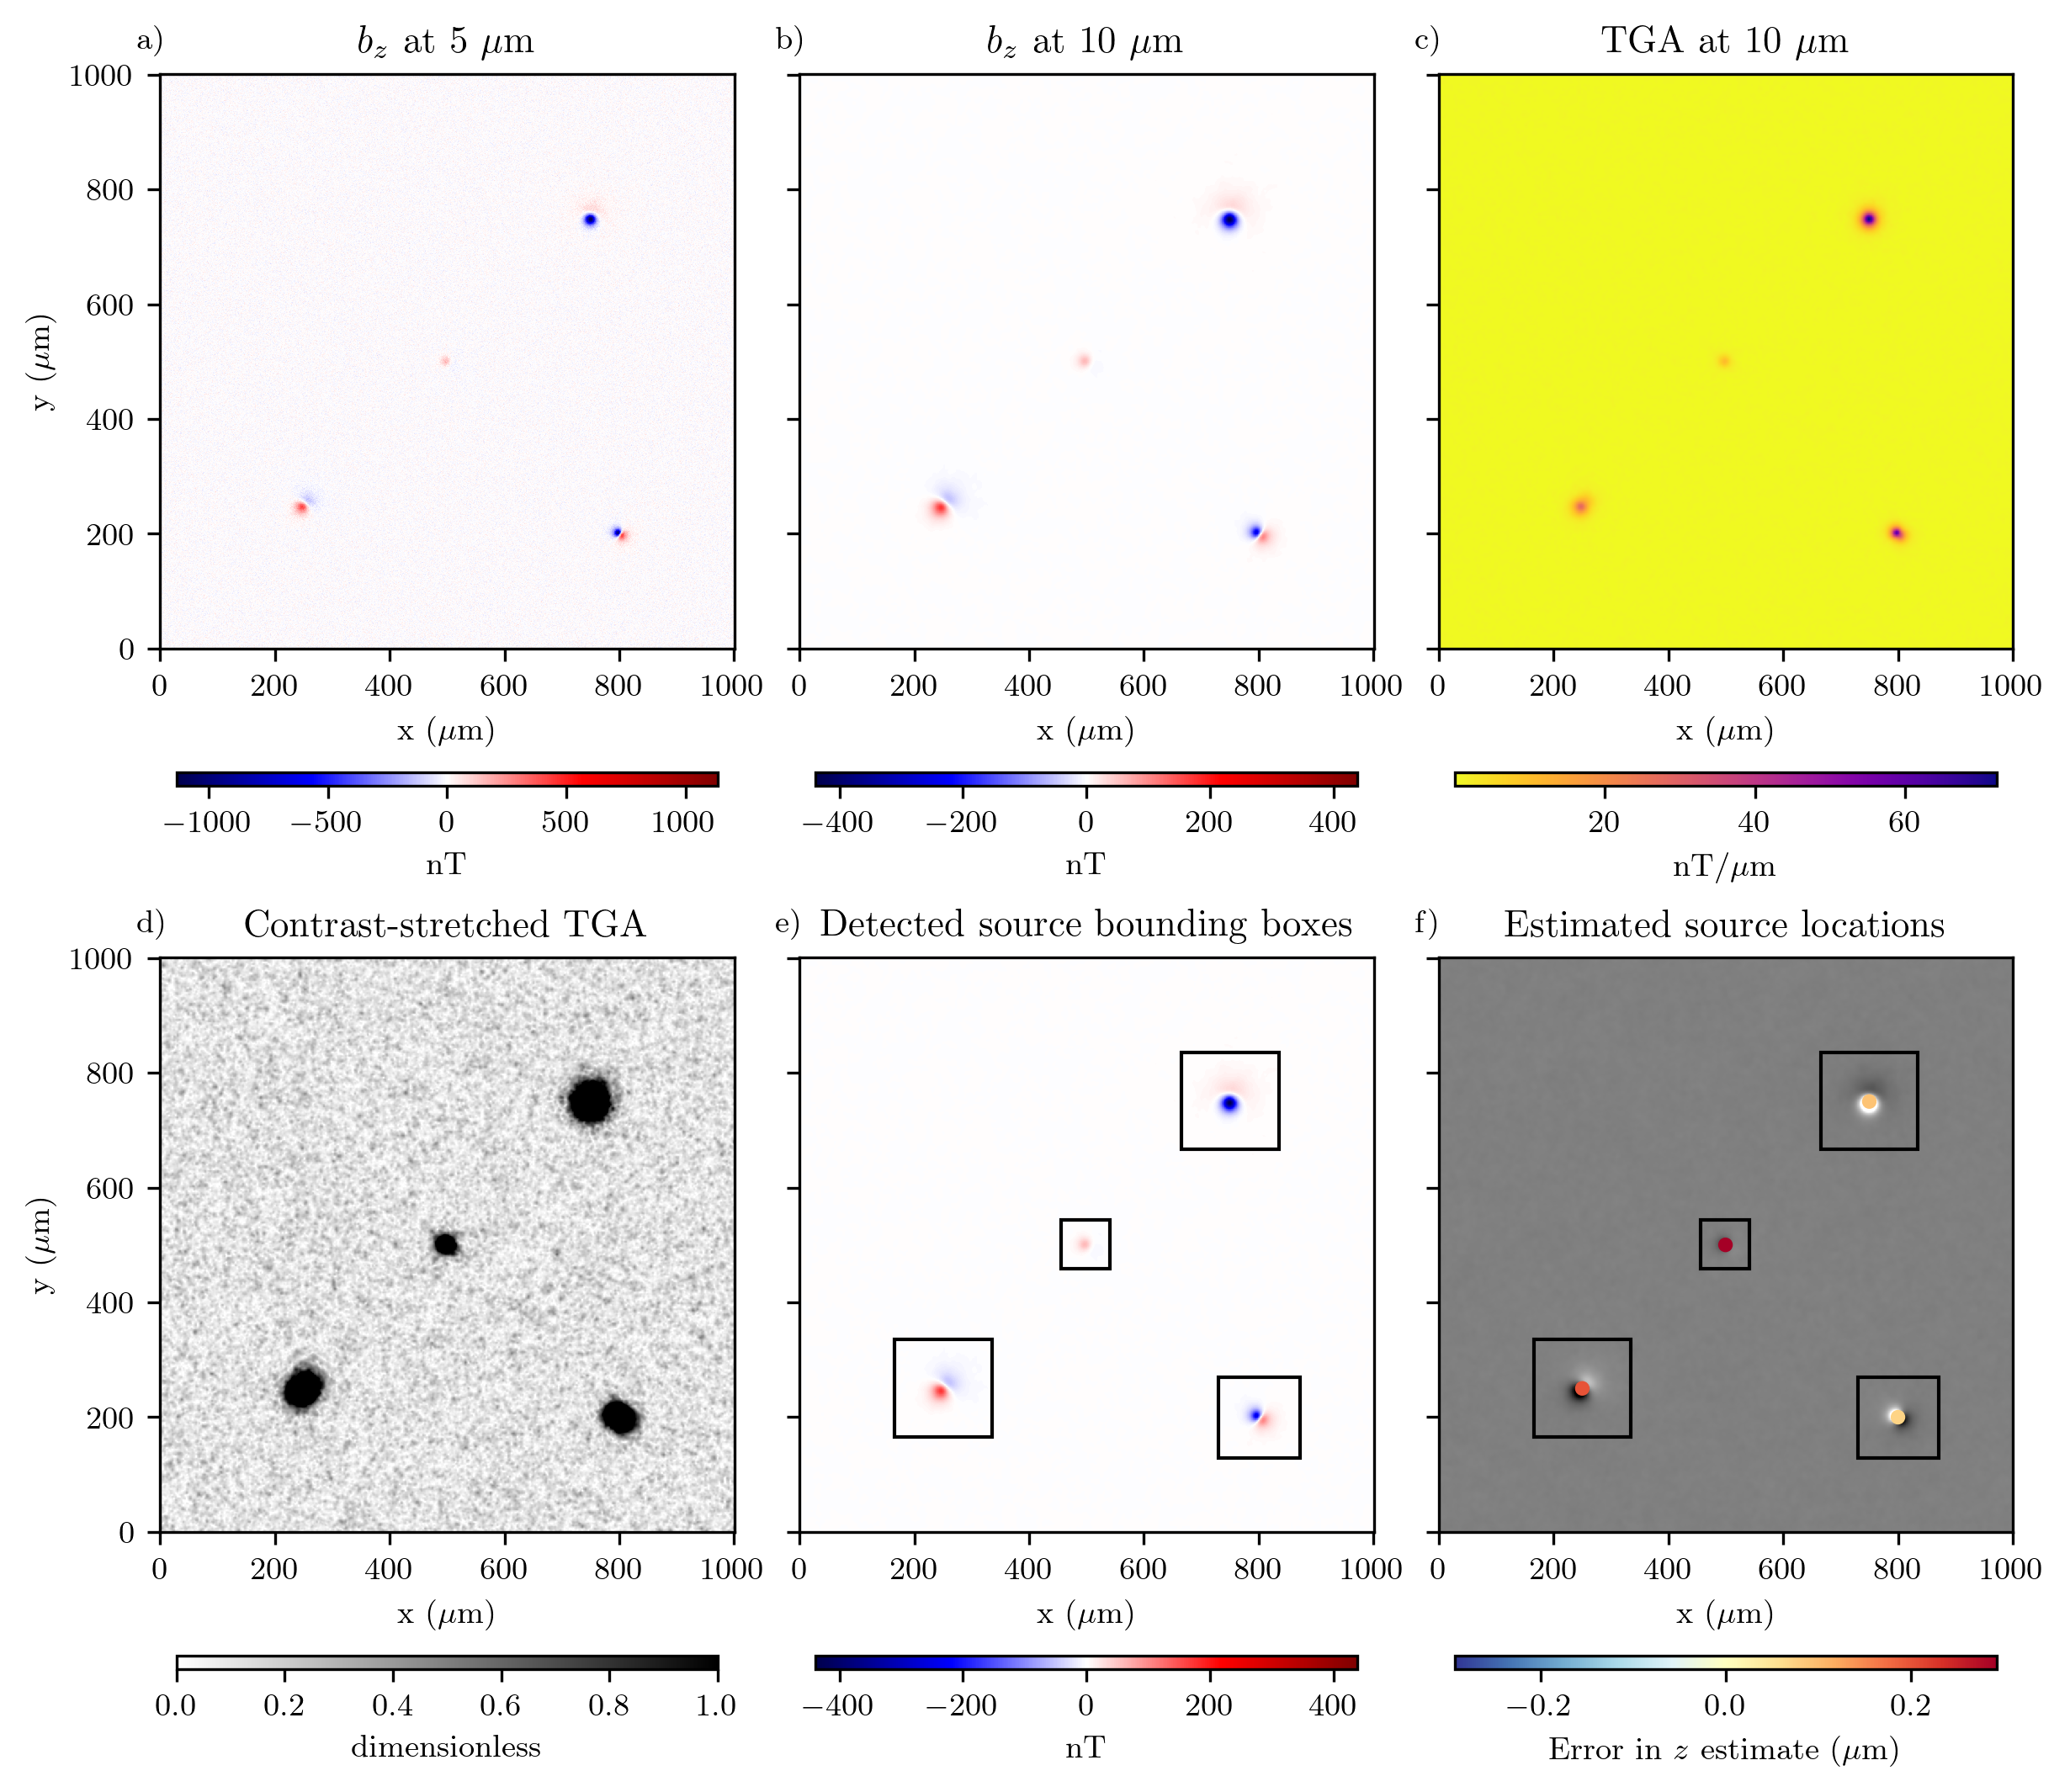
\includegraphics[width=1\linewidth]{figures/simple-synthetic-data.png}
  \caption{
    Simple synthetic data and the various processing steps performed prior to the dipole moment inversion.
    a) The synthetic noise-corrupted $b_z$ observations at
    $z = \qty{5}{\micro\meter}$ due to four dipolar sources with different
    depths and dipole moment vectors
    (see Table~\ref{tab_synthetic_simple_results}).
    b) The upward-continued data to $z = \qty{10}{\micro\meter}$ showing
    attenuated short-wavelength noise.
    c) The total gradient amplitude (TGA) calculated from the
    upward-continued data, which is able to concentrate the signal on top
    of each dipolar source.
    d) The contrast-stretched TGA, highlighting the signal of all four
    sources, including the weak central source.
    e) The detected source bounding boxes (black squares) that correctly
    identify the signal of all four sources.
    f) The estimated source locations (colored circles) from Euler
    Deconvolution of the upward-continued data inside each bounding box.
    The color represents the difference between the true and estimated
    $z$ coordinates.
  }
  \label{fig_synthetic_simple_data}
\end{figure}

Figure~\ref{fig_synthetic_simple_data}a shows the vertical component of the magnetic field $b_z$ over a synthetic rock section containing four dipolar sources.
The map covers a surface of $\qty{1000}{\um} \times \qty{1000}{\um}$, with data points in a regular grid with approximately \qty{1}{\um} spacing ($N = 10^6$ observations) obtained at a sensor-sample distance of \qty{5}{\um}.
The magnetic field data are contaminated with pseudo-random Gaussian noise with zero mean and \qty{20}{\nano\tesla} standard deviation.

We first applied an upward continuation filter (Figure~\ref{fig_synthetic_simple_data}b) to smooth out the high-frequency noise \citep{Blakely1996}.
This is important because it strongly affects the first derivatives of the field, which are required for the Euler Deconvolution.
Then, we calculated the total gradient amplitude (Figure~\ref{fig_synthetic_simple_data}c), which was then subjected to contrast stretching to highlight as much as possible the weaker intensity sources (Figure~\ref{fig_synthetic_simple_data}d).
Subsequently, we applied the blob detection algorithm to the contrast-stretched total gradient amplitude to obtain the position of the data windows for each source (Figure~\ref{fig_synthetic_simple_data}e).
Euler Deconvolution was then performed for each data window identified by assuming a structural index $\eta = 3$ of a point source, therefore obtaining the Cartesian coordinates (Figure~\ref{fig_synthetic_simple_data}f) of each source. Table~\ref{tab_synthetic_simple_results} shows the true and estimated values of the source coordinates for comparison.

\begin{figure}[tb!]
\centering
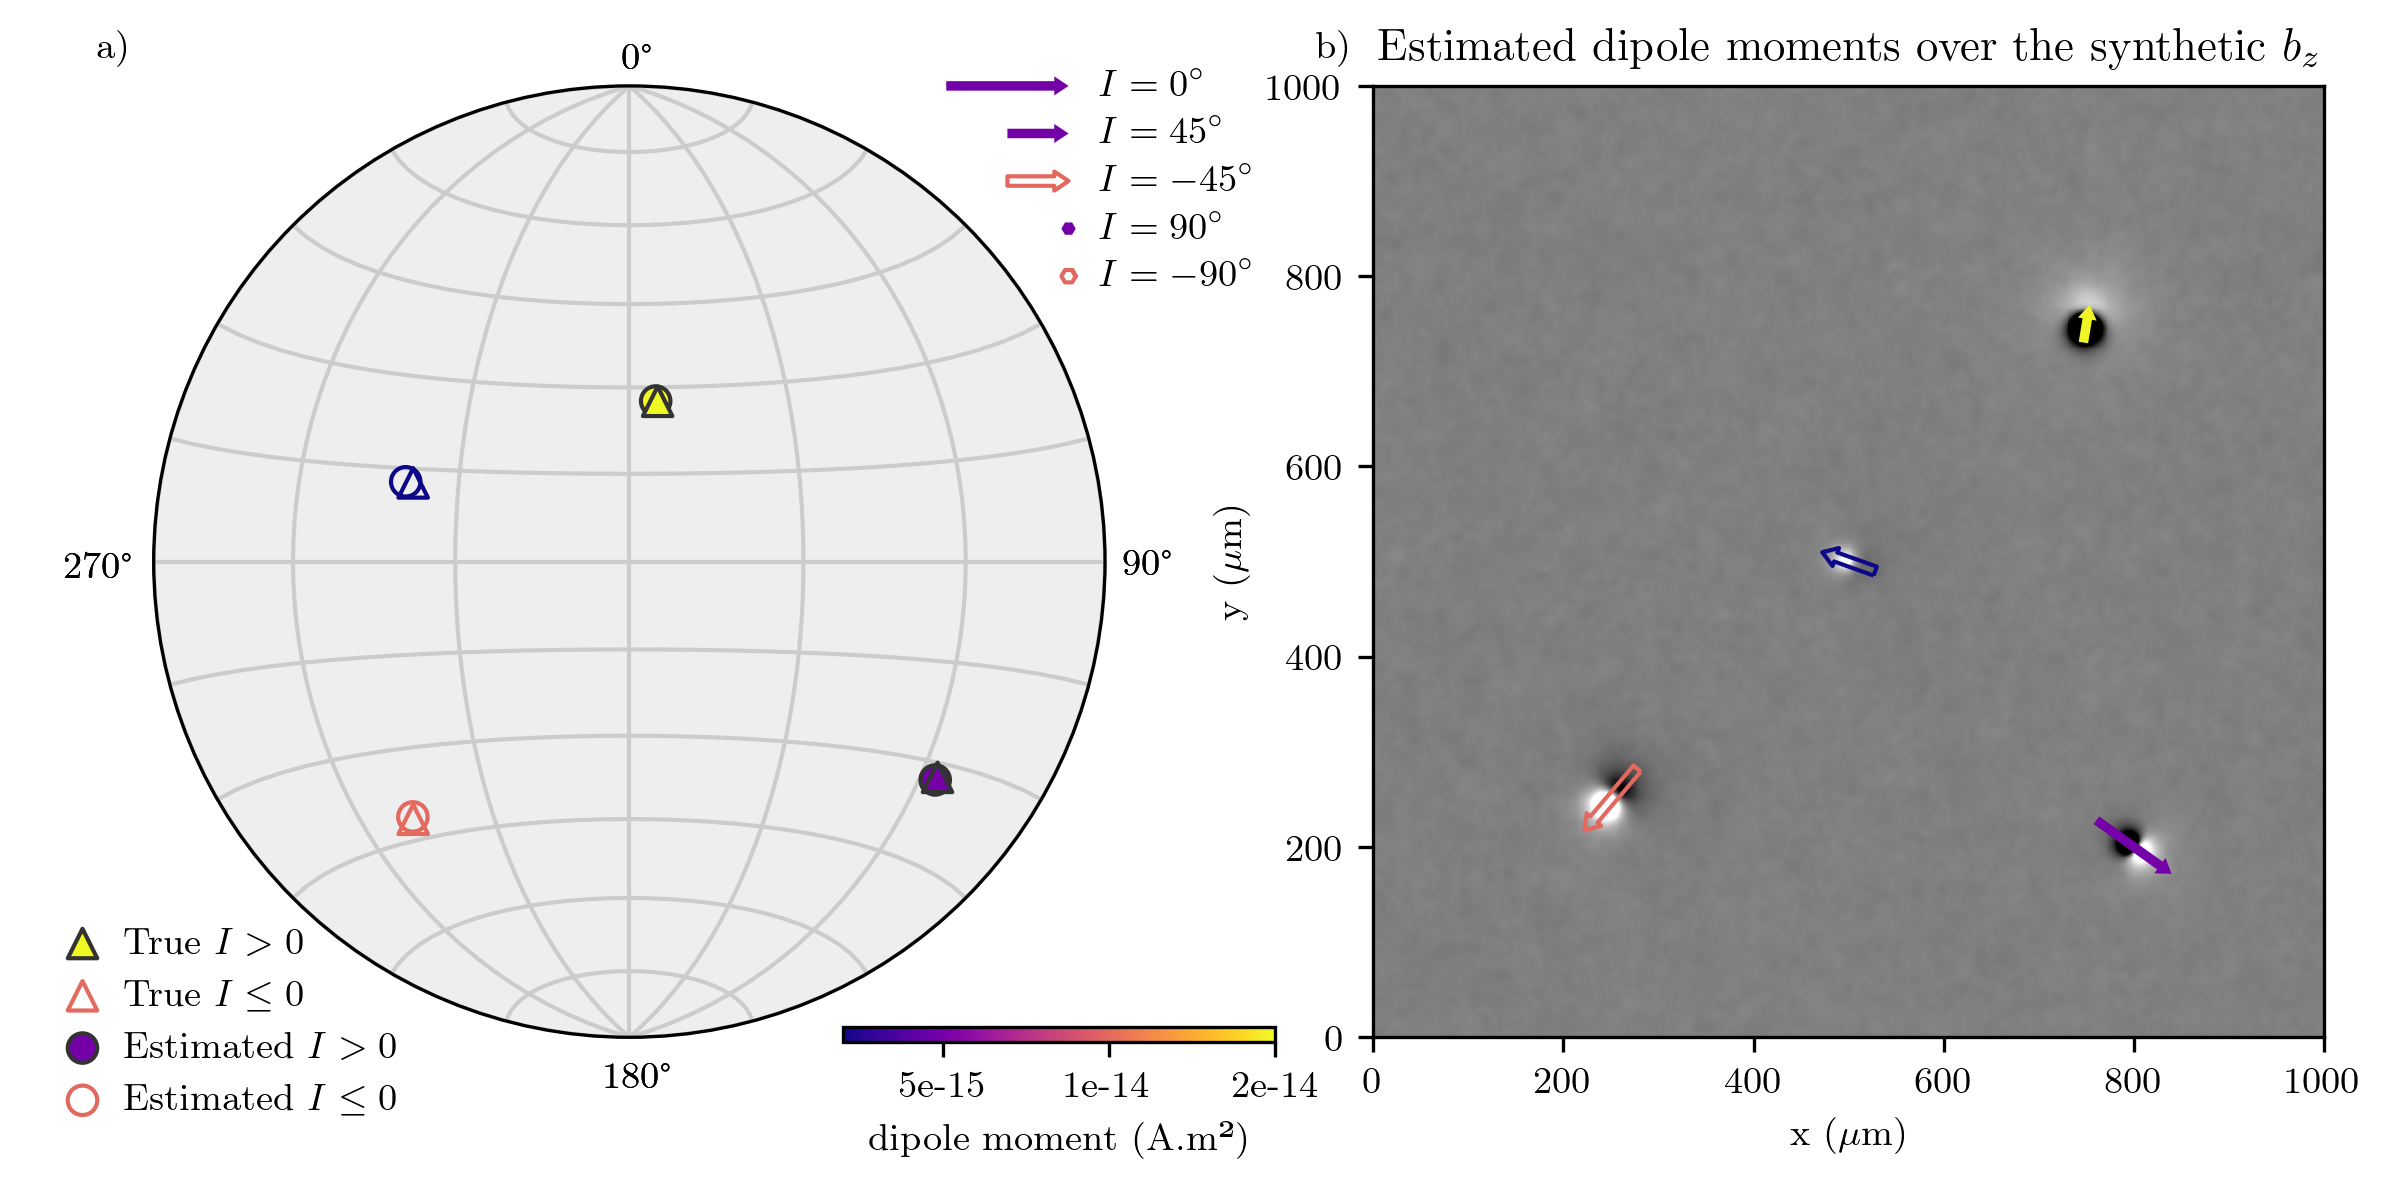
\includegraphics[width=\linewidth]{figures/simple-synthetic-dipole-moment.png}
\caption{
Comparison of true and estimated dipole magnetic moments and directions.
}
\label{fig_synthetic_simple_results}
\end{figure}

The positions of each source obtained with Euler deconvolution were used as an input parameter for the dipole moment inversion.
The estimated inclination ($I$), declination ($D$), and dipole moment amplitude ($m$) are shown in Figure~\ref{fig_synthetic_simple_results} along with the corresponding true values.
Table~\ref{tab_synthetic_simple_results} also shows the true and estimate dipole moments as well as their corresponding standard deviations obtained using Equations~\ref{eq_chi_square}-\ref{eq_variances}.

\begin{table}[tb]
  \begin{center}
    \small
    
\begin{tabular}{ r c c c l l l } 
  \toprule
  & \multicolumn{3}{c}{Position} & \multicolumn{3}{c}{Dipole moment} \\
  & $x_c$ ($\mu$m) & $y_c$ ($\mu$m) & $z_c$ ($\mu$m) & $I$ (\textdegree) & $D$ (\textdegree) & $m$ (A.m²) \\
  \midrule
  true & 800.00 & 200.00 & -3.50 & 22.00 & 125.00 & 5.000e-15 \\
  estimated & 799.91 & 199.94 & -3.40 & 22.08 ± 0.01 & 125.52 ± 0.02 & 4.921e-15 ± 1.4e-18 \\
  true & 750.00 & 750.00 & -8.50 & 62.00 & 10.00 & 1.500e-14 \\
  estimated & 749.98 & 749.99 & -8.43 & 62.00 ± 0.01 & 9.30 ± 0.02 & 1.486e-14 ± 1.8e-18 \\
  true & 250.00 & 250.00 & -10.00 & -30.00 & -140.00 & 1.000e-14 \\
  estimated & 250.03 & 249.89 & -9.93 & -30.32 ± 0.01 & -139.70 ± 0.02 & 9.966e-15 ± 2.6e-18 \\
  true & 500.00 & 500.00 & -7.75 & -50.00 & -70.00 & 2.000e-15 \\
  estimated & 500.07 & 499.95 & -7.76 & -48.66 ± 0.05 & -70.36 ± 0.09 & 2.000e-15 ± 1.8e-18 \\
  \bottomrule
\end{tabular}

  \end{center}
  \caption{
  True and estimated source positions and dipole moments for the simple synthetic data application.
  Each source modeled and recovered positioning and magnetization parameters by the least square estimator, respectively.}
  \label{tab_synthetic_simple_results}
\end{table}


\subsection{Simple simulation: Validating the methodology for non-dipolar sources}

Typically, when conducting magnetic field measurements with a large distance between the sensor and the magnetic anomaly source, higher-order non-dipole magnetization components such as quadrupoles and octupoles are disregarded. However, in magnetic microscopy, where the sensor is positioned very close to the sample, these higher-order components might be detected. This phenomenon is observed in paleomagnetic studies on particles with a PSD domain state, where magnetization is non-uniform throughout the grain. To assess the magnetic signal attenuation, simulations were conducted on particles with more complex magnetization at varying distances from the sensor.

To simulate particles with non-dipole magnetization components, we specified a spherical volume with a radius of about 1 $\mu$m. Within this volume, we added 200 dipolar point particles with varying magnetization directions and magnetic moments. These directions were generated randomly to follow a normal distribution centered on the direction Dec=90°/Inc=0°, with a magnetic moment of $10^{-14}$ Am$^2$. We also randomly generated the spatial positions around a central position of $x_c=25~\mu$m, $y_c=25~\mu$m, and $z_c=\alpha~\mu$m, where $\alpha$ = 0, 1, ... 11 corresponds to the variation in depth of the particle. By summing the $m_x$, $m_y$, and $m_z$ components of each modeled particle, we obtained the Cartesian magnetization components for the spherical particle. The centroid of the particle was defined by the average of the $x_c$, $y_c$, and $z_c$ positions. The modeled vertical magnetic field was corrupted by a random noise of mean zero and a standard deviation of 20 nT.

According to Figure~\ref{non-dipolarity-synthetic-data} obtained from this simulation, it can be observed that when the particle is very close to the sensor, there is a strong non-dipolar contribution (Figure~\ref{non-dipolarity-synthetic-data}a-b) characterized by low $R^2$ values, indicating low dipolarity. As the distance increases, the magnetic signal is strongly attenuated, especially the non-dipolar components that decay more rapidly than the dipolar component, resulting in a rapid increase in $R^2$ (Figure~\ref{non-dipolarity-synthetic-data}c-d). At distances above 5 $\mu$m, there is practically only the contribution of the dipolar component, causing $R^2$ values to be very close to 1 (Figure~\ref{non-dipolarity-synthetic-data}e-f).

\begin{figure}[tb!]
  \centering
  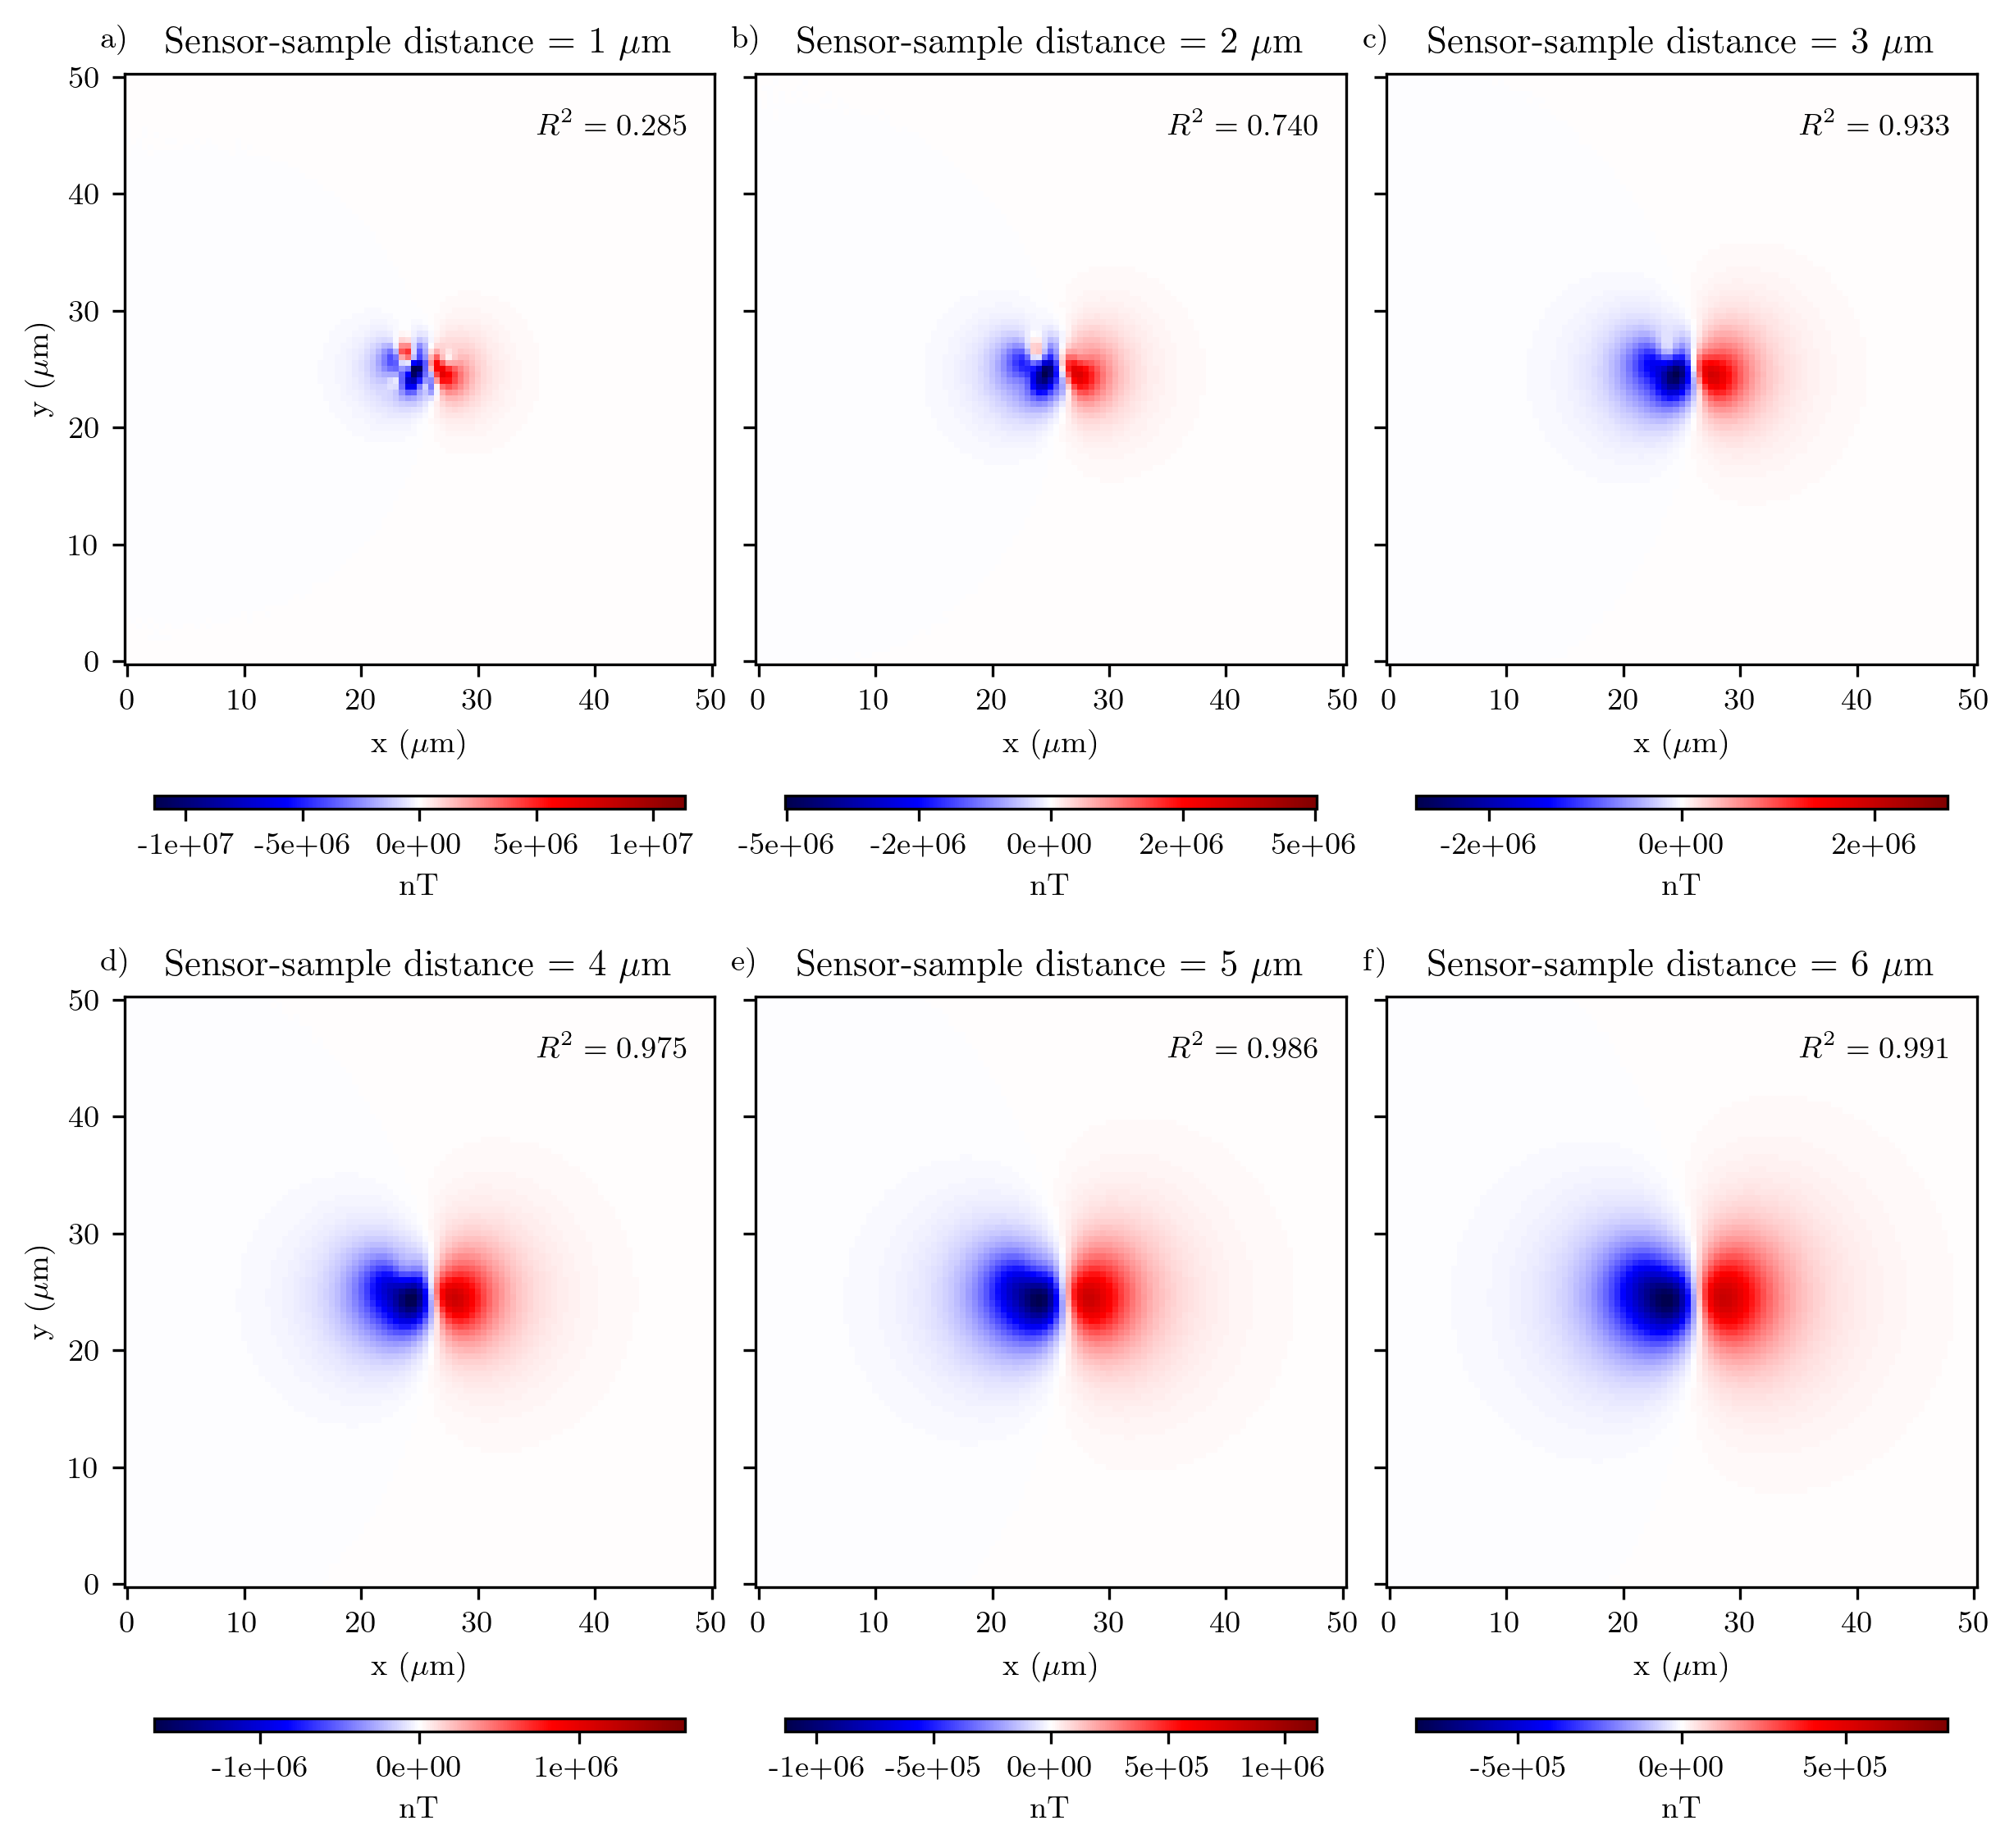
\includegraphics[width=1\linewidth]{paper/figures/non-dipolarity-synthetic.png}
  \caption{Caption: Simulated magnetic microscopy data for a spherical source with both dipolar and non-dipolar magnetic components. The distance from the sensor varies from 1 µm to 6 µm (a-f).}
  \label{non-dipolarity-synthetic-data}
\end{figure}


To assess the algorithm's capability to handle particles with more complex magnetization, we replicated the particle generation procedure 100 times with variations in the randomness of magnetization and point particle positions. Subsequently, the Cartesian position of the spherical particle was estimated using ED, and the magnetization parameters were determined by inverting the magnetic field data. The effectiveness of position recovery was measured by comparing the particle's centroid with the solution of the Euler equation for $x_c$, $y_c$, and $z_c$ (Figure~\ref{non-dipolarity-synthetic-data-positioning}a, b, and c, respectively). As shown in Figure~\ref{non-dipolarity-synthetic-data-positioning}, ED estimates the positions of particles with more complex magnetization well, especially for sensor-source distances greater than 5 µm, where the median of the distributions is centered at zero. However, when the sensor-source distance is small enough for there to be a strong contribution from higher-order components, a lower degree of dipolarity is observed, expressed as lower values of $R^2$ (Figure~\ref{non-dipolarity-synthetic-data-inversion}a). Consequently, in these cases, there are higher errors in the direction of magnetization (Figure~\ref{non-dipolarity-synthetic-data-inversion}b) and in the magnetic moment's intensity (Figure~\ref{non-dipolarity-synthetic-data-inversion}c), which was expected since the inversion considers only the dipolar component. However, dipolarity significantly increases as the sensor distance increases, while errors in direction and magnetic moment decrease significantly (Figure~\ref{non-dipolarity-synthetic-data-inversion}).

\begin{figure}[tb!]
  \centering
  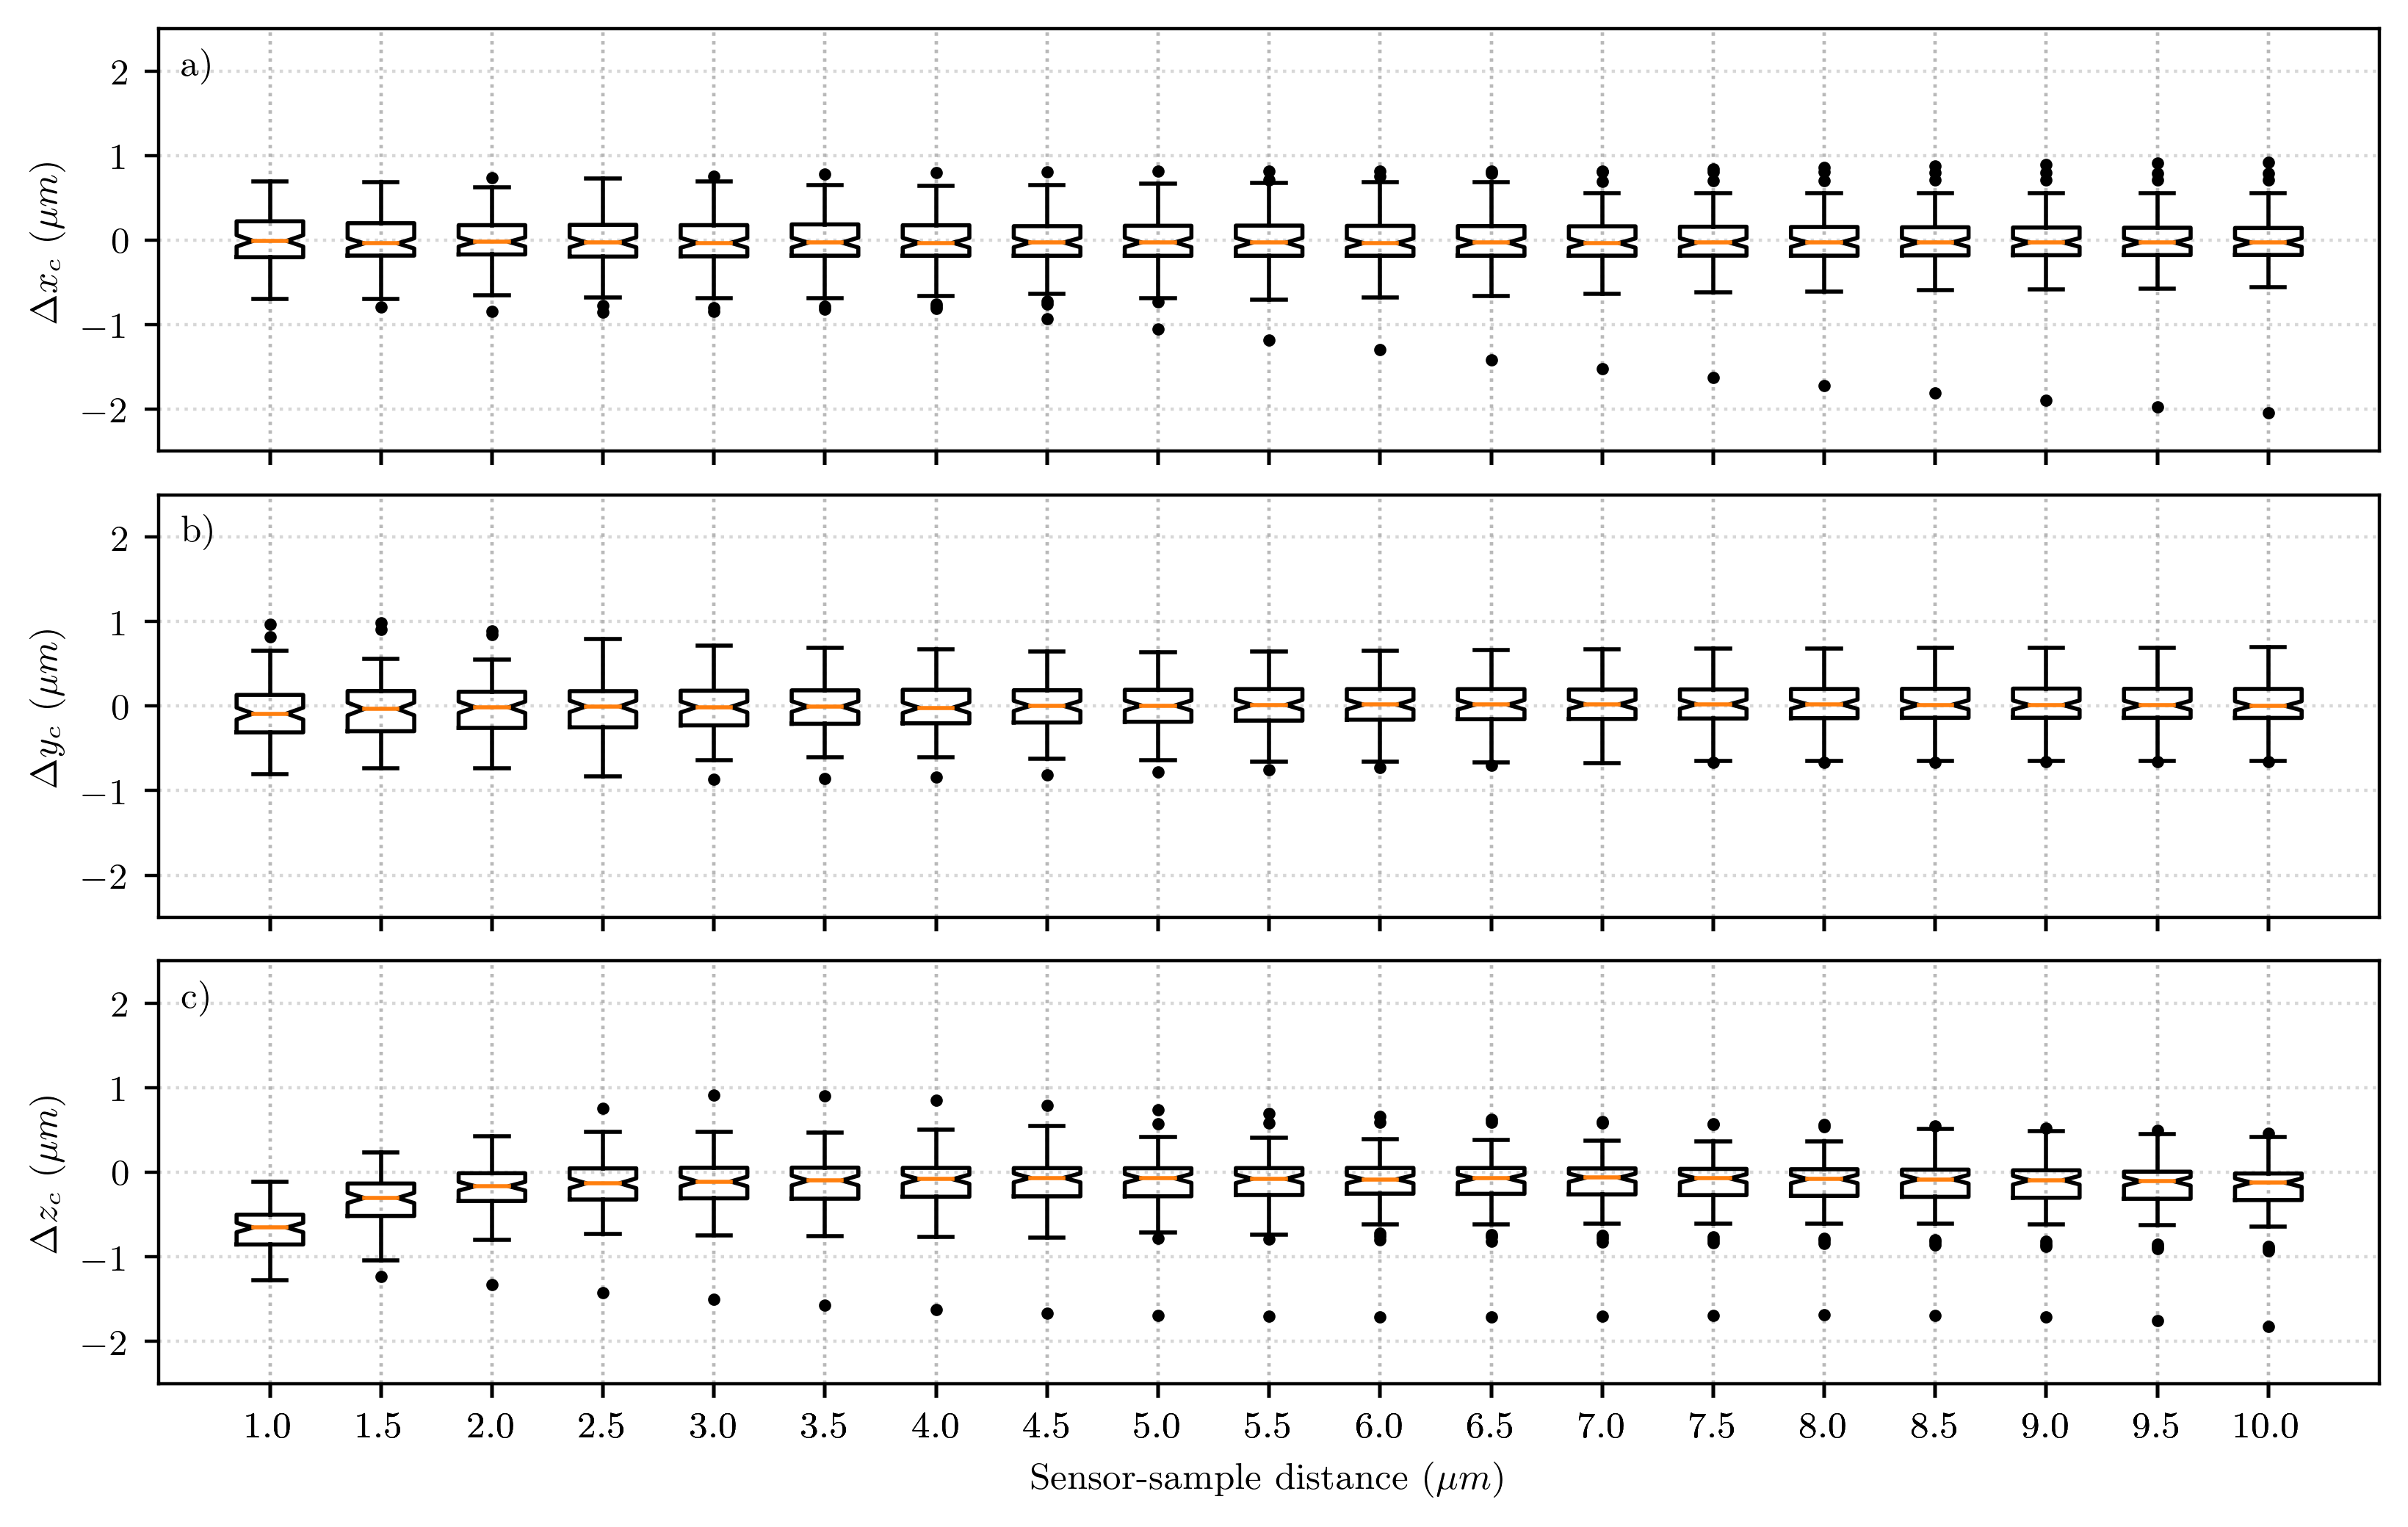
\includegraphics[width=1\linewidth]{paper/figures/non-dipolarity-synthetic-positioning.png}
  \caption{The simulation was randomly replicated (N=100) to test the effectiveness of the Euler deconvolution in estimating the position of the modeled particles. The difference between the true position (centroid) and the estimated position was calculated for each replicate and plotted as a boxplot. The boxplot shows the distribution of differences in the (a) $x_c$, (b) $y_c$, and (c) $z_c$.}
  \label{non-dipolarity-synthetic-data-positioning}
\end{figure}

\begin{figure}[tb!]
  \centering
  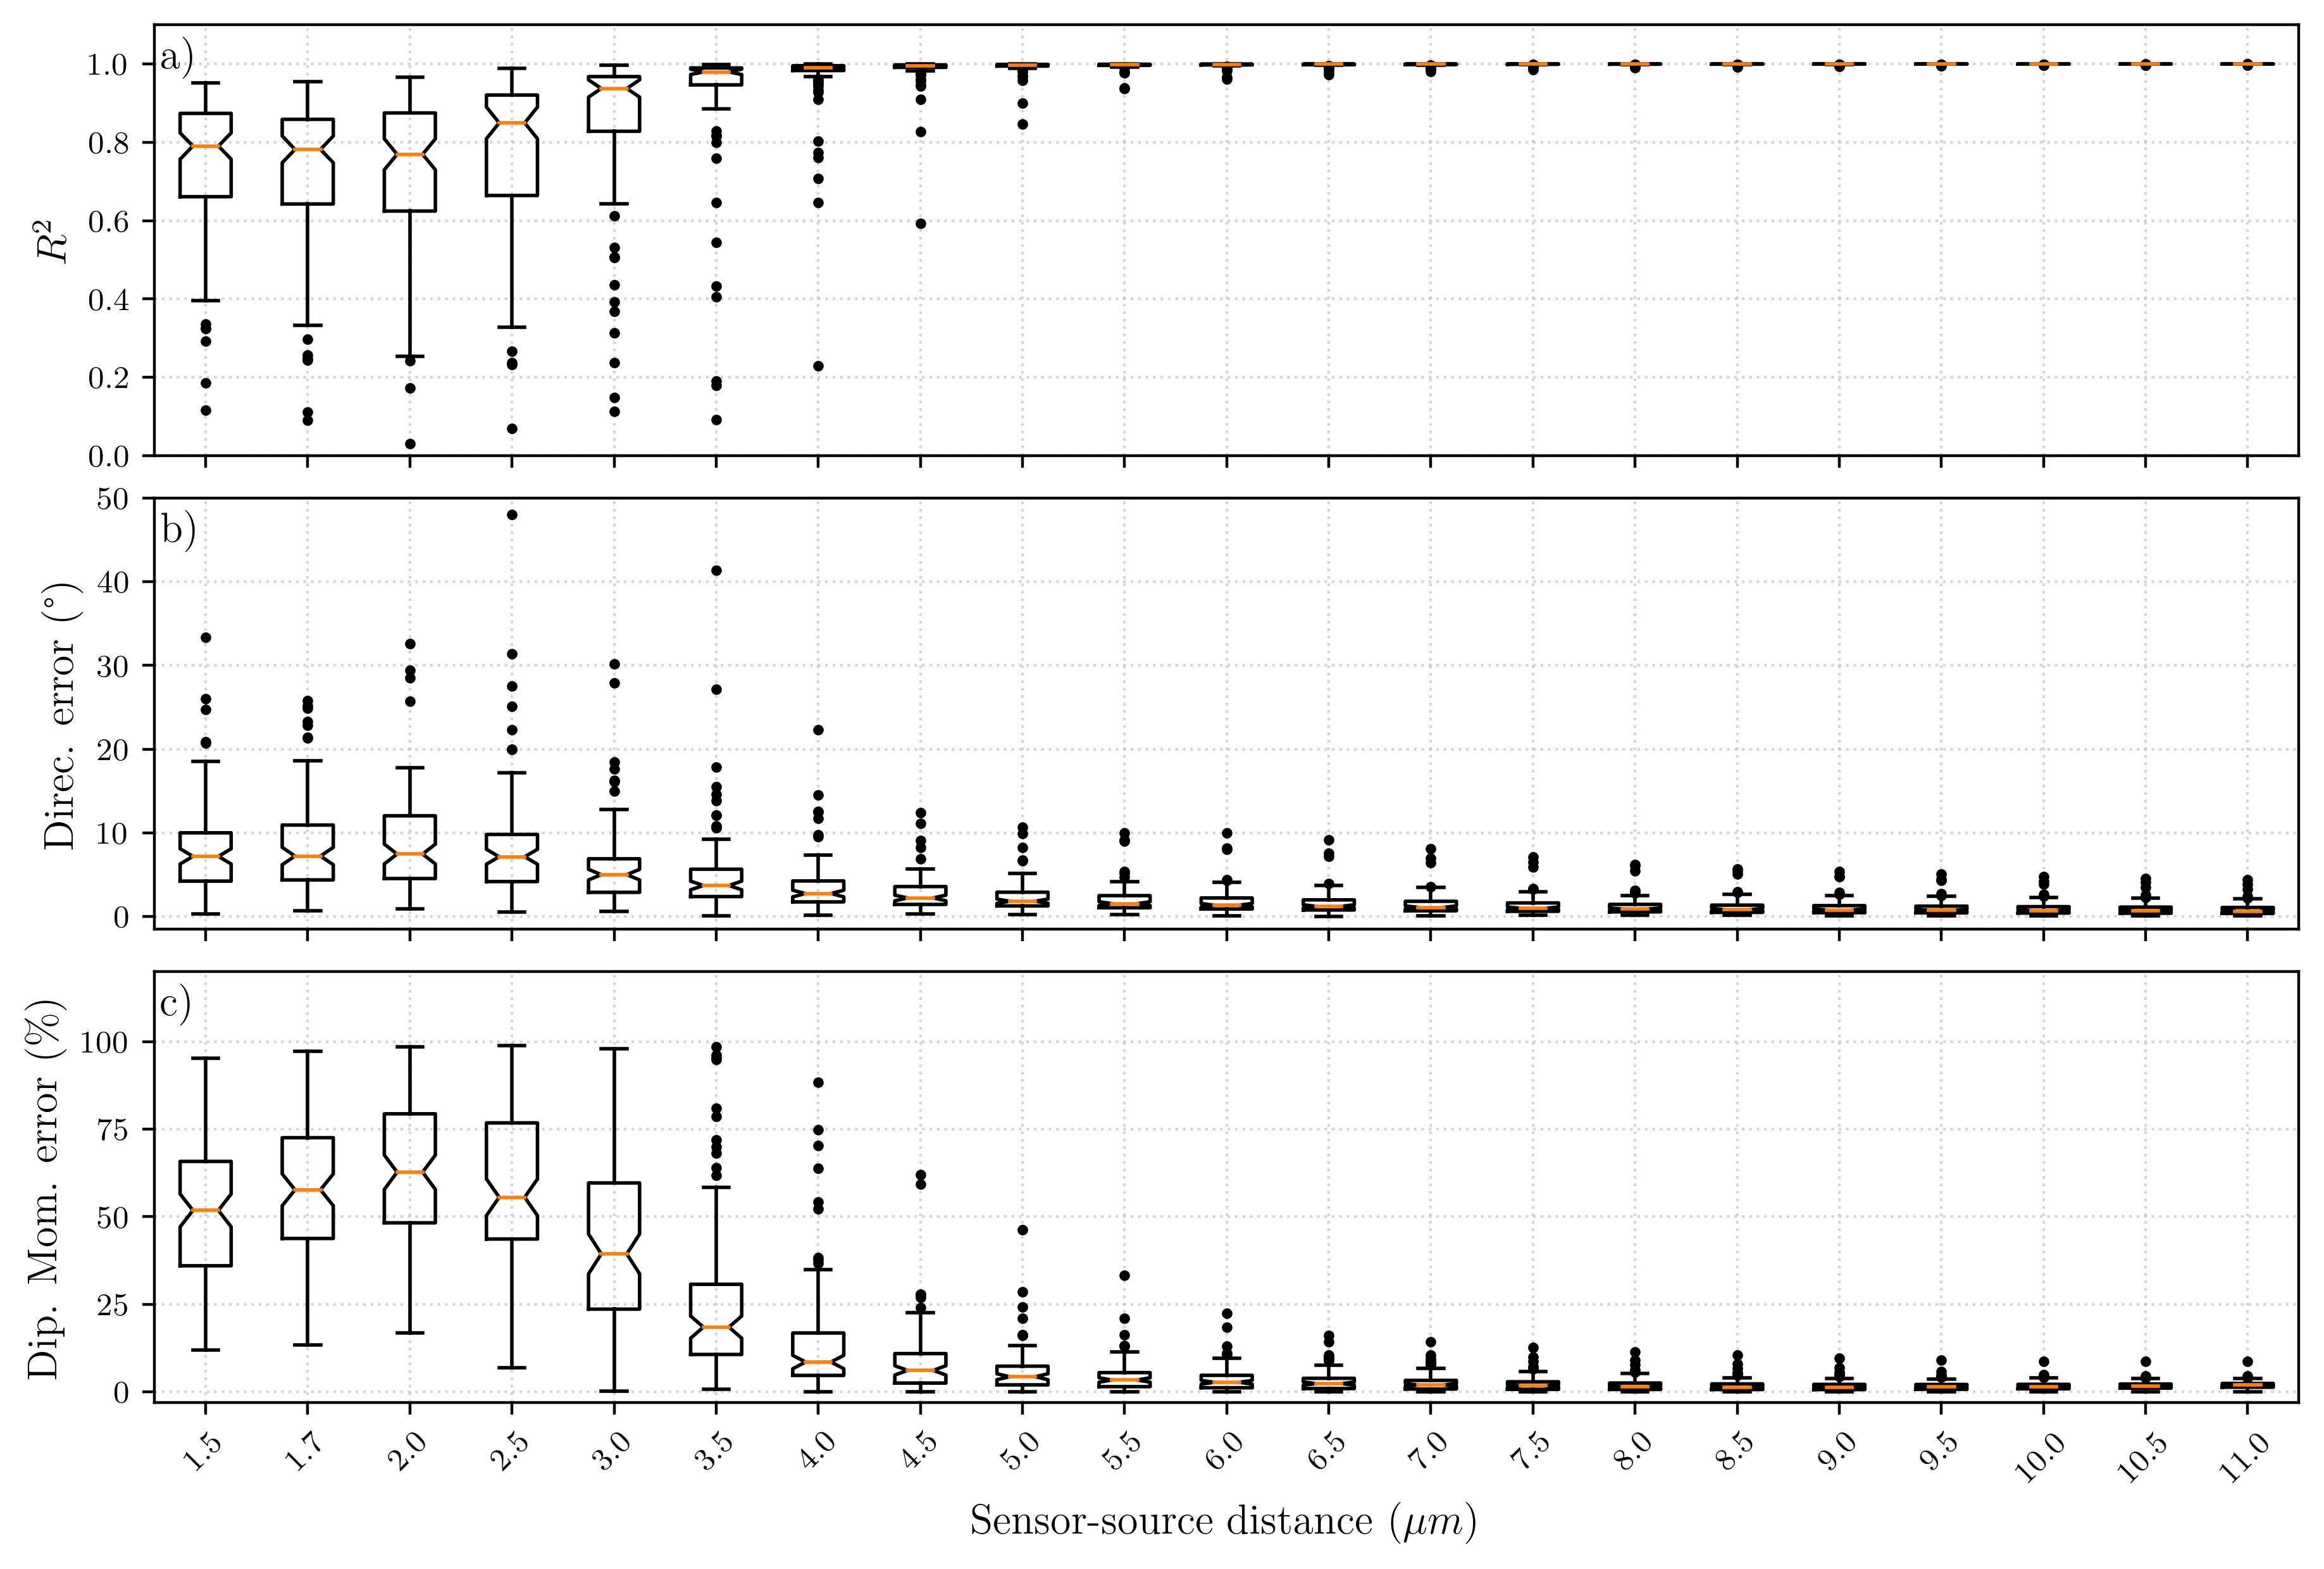
\includegraphics[width=1\linewidth]{paper/figures/non-dipolarity-synthetic-inversion.png}
  \caption{The simulation was randomly replicated (N=100) to assess the accuracy of the algorithm in recovering the magnetic direction and moment of the modeled particles. The goodness of fit was measured by the R-squared value (a), while the angular error (b) and intensity error (c) between the real and modeled magnetic vector were plotted in degrees and percentages ($|100 \left( m_{true} - m_{estimated}\right) ~/~ m_{true}|$), respectively.}
  \label{non-dipolarity-synthetic-data-inversion}
\end{figure}



\subsection{Complex simulation: Testing applicability}

This test represents a more complex scenario by simulating 103 sources randomly distributed in the imaged area of a synthetic thin section of $\qty{2000}{\um} \times \qty{2000}{\um}$.
The synthetic $b_z$ data were generated on a regular grid with $\qty{2}{\um}$ spacing and $\qty{5}{\um}$ sensor-sample distance.
We contaminated the data with high-frequency normally-distributed pseudo-random noise with zero mean and $\qty{50}{\nano\tesla}$ standard deviation, as well as with low-frequency noise in the form of additional deep sources beyond the modeling domain.

For greater fidelity to real samples, the magnetic sources are modeled as dipoles with different depths and magnetic moment intensities.
The depths vary randomly between 1 and $\qty{20}{\um}$, while the dipole moment intensities range randomly from $10^{-12}$ to $\qty{e-14}{\ampere\m\squared}$.
The NRM found in real ferromagnetic particles varies individually but averages out to the inducing field direction.
To simulate this behavior in our synthetic data, we sample the source dipole moment directions from two pseudo-random Gaussian distributions.
The first group of sources ($M = 70$) are sampled from a distribution  with mean of $D = \ang{0}$ and $I = \ang{0}$ and standard deviation of $\ang{10}$.
The second group of sources ($M = 30$) are sampled from a distribution with mean of $D = \ang{180}$ and $I = \ang{0}$, also with standard deviation of $\ang{10}$. We also manually added 3 sources with higher dipole moments ($5x10^{-11}$) to further simulate the complexity observed in real data measurements. The noise-corrupted synthetic $b_z$ data are shown in Figure~\ref{complex-synthetic-data}a.

\begin{figure}[tb!]
  \centering
  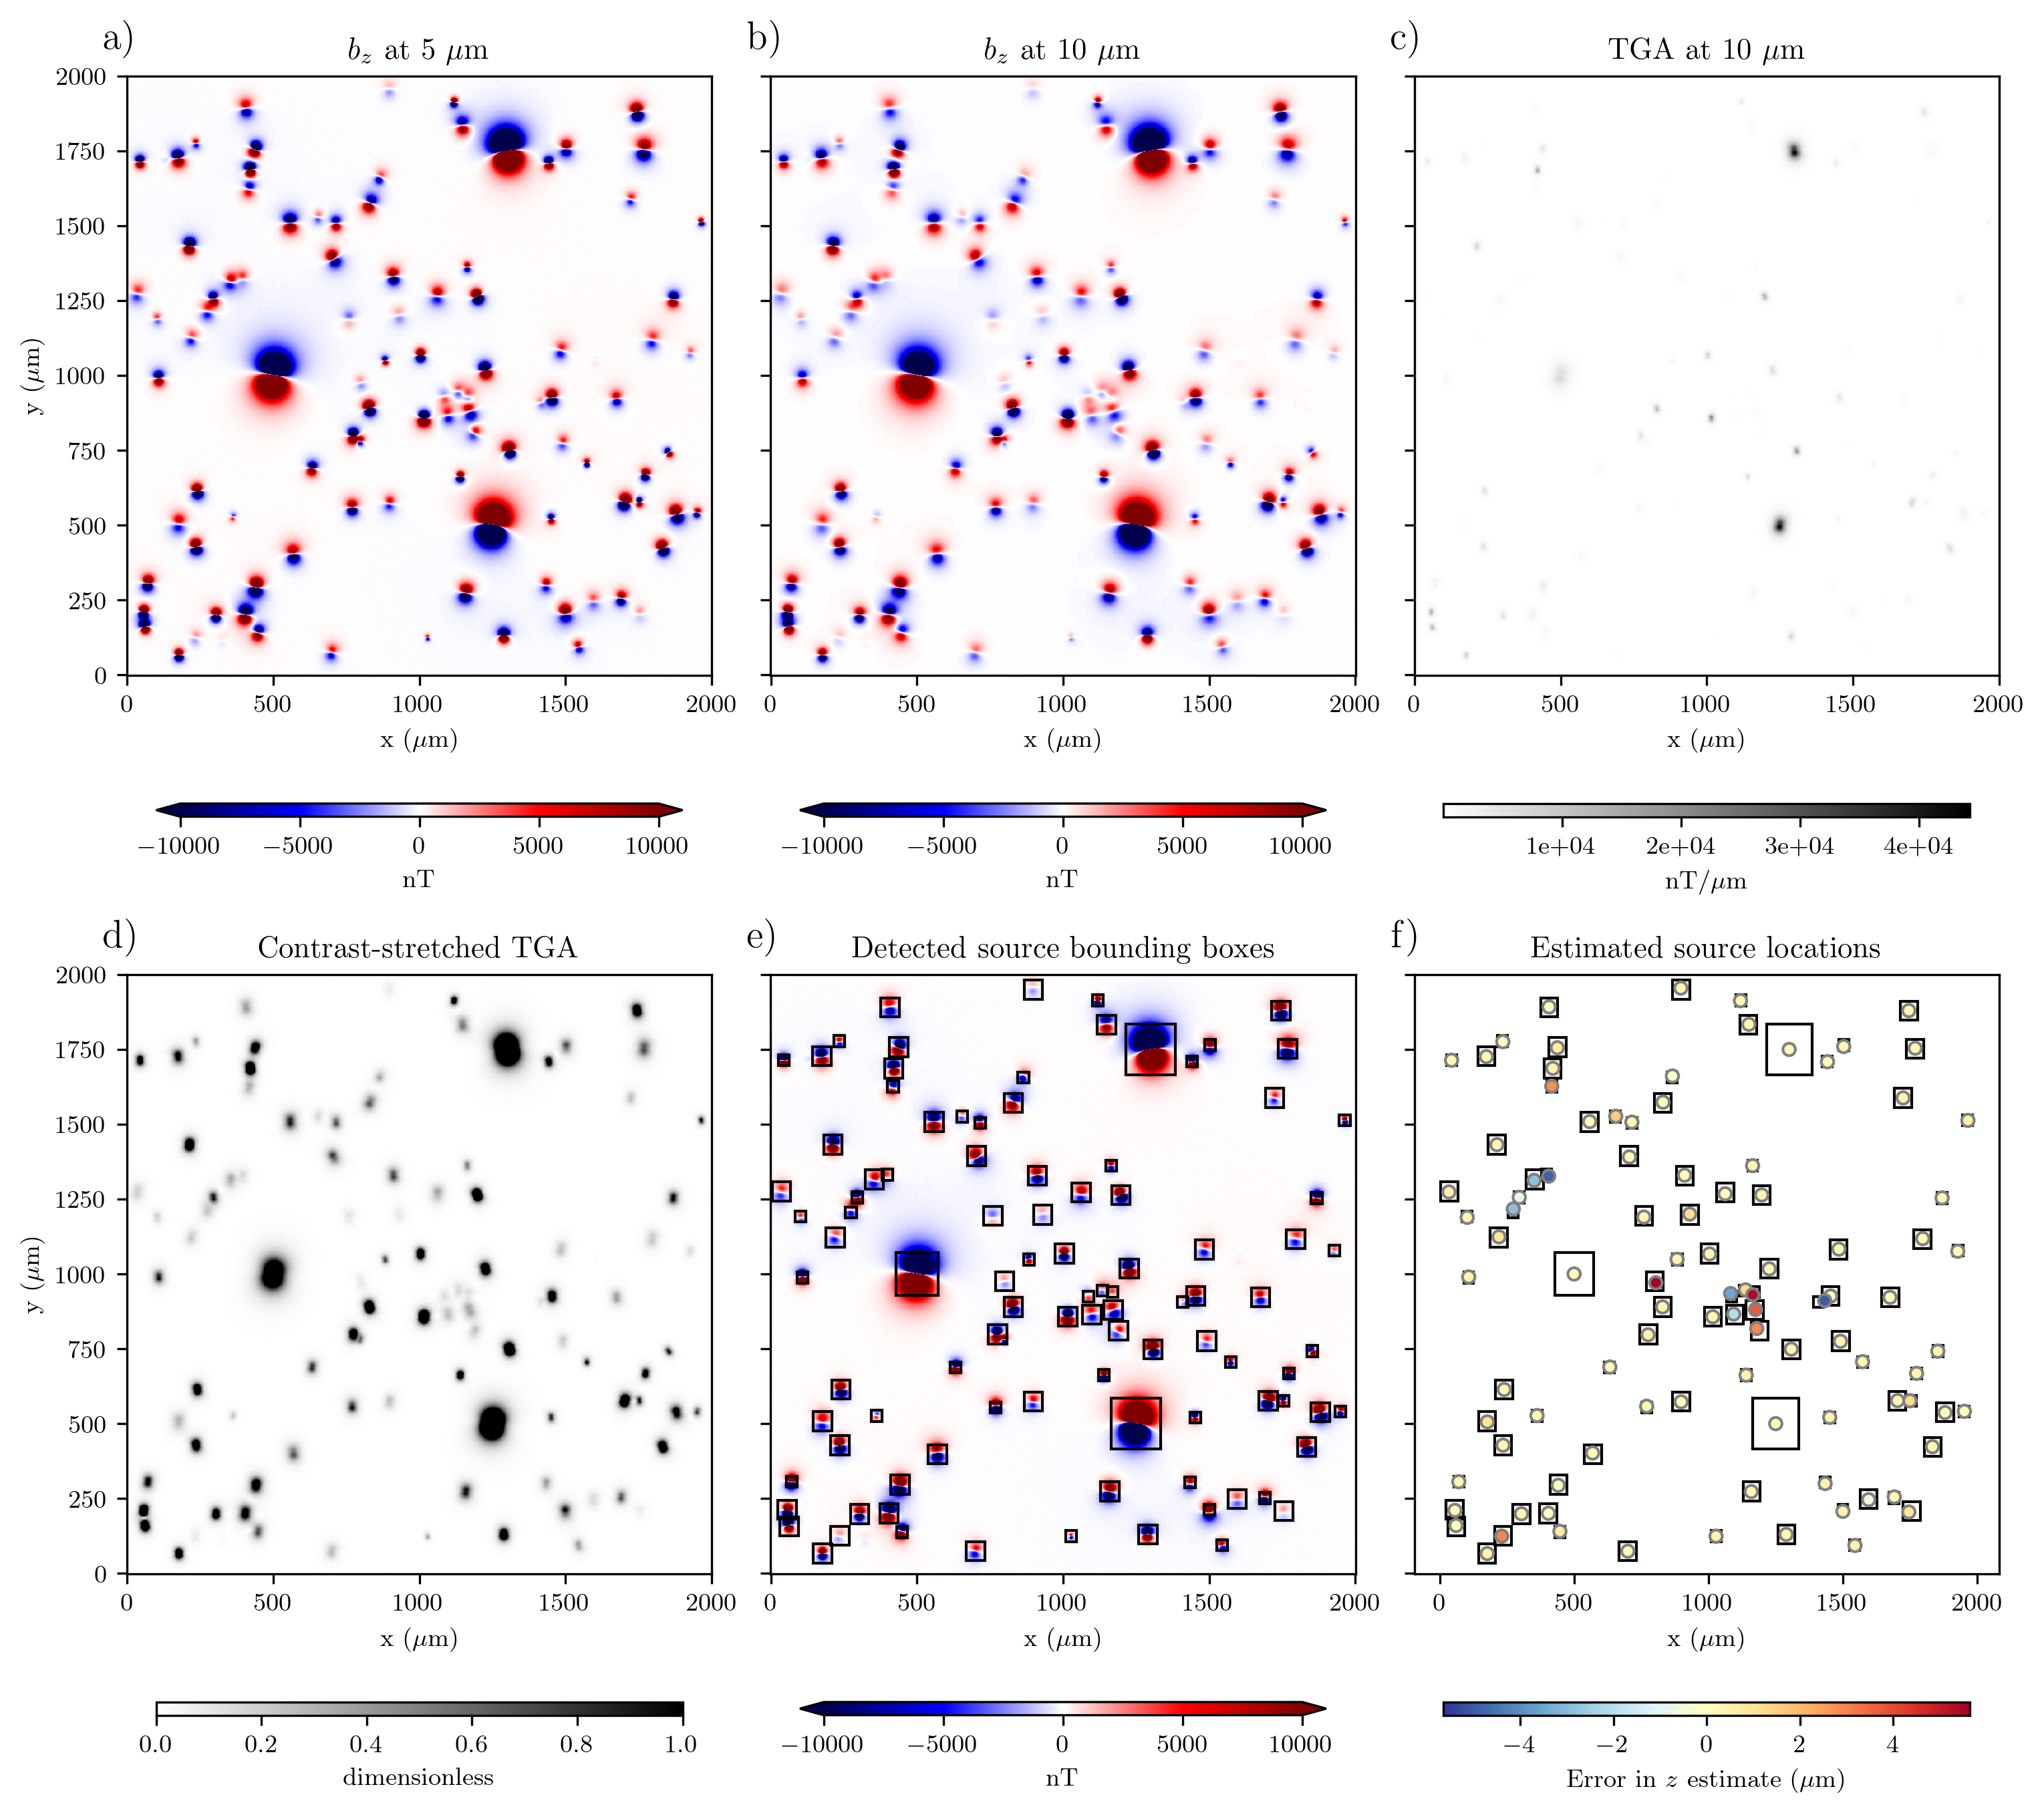
\includegraphics[width=1\linewidth]{figures/complex-synthetic-data.png}
  \caption{
    Complex synthetic data and the various processing steps performed prior to the dipole moment inversion.
    a) The synthetic high and low-frequency noise-corrupted $b_z$ observations at
    $z = \qty{5}{\micro\meter}$ due to two clusters of stable directions simulated.
    b) Anomaly map after the upward-continued data to $z = \qty{10}{\micro\meter}$ to attenuated long and short-wavelength noise.
    c) The total gradient amplitude (TGA) calculated from the
    upward-continued data, which is able to concentrate the signal on top
    of each dipolar source.
    d) The contrast-stretched TGA, highlighting the signal of all sources, especially the weaker ones.
    e) The detected source bounding boxes (black squares) that correctly
    encapsulate the signal of the sources.
    f) The estimated source locations (colored circles) from Euler
    Deconvolution of the upward-continued data inside each bounding box.
    The color represents the difference between the true and estimated
    $z$ coordinates.
  }
  \label{complex-synthetic-data}
\end{figure}

We then followed the same processing steps as for the simple synthetic: upward continuation (Figure~\ref{complex-synthetic-data}b),
TGA calculation (Figure~\ref{complex-synthetic-data}c), contrast stretching (Figure~\ref{complex-synthetic-data}d), blob detection (Figure~\ref{complex-synthetic-data}e), and Euler Deconvolution (Figure~\ref{complex-synthetic-data}e).
A total of 99 sources out of the original 103 were successfully detected by our workflow.

\begin{figure}[tb!]
\centering
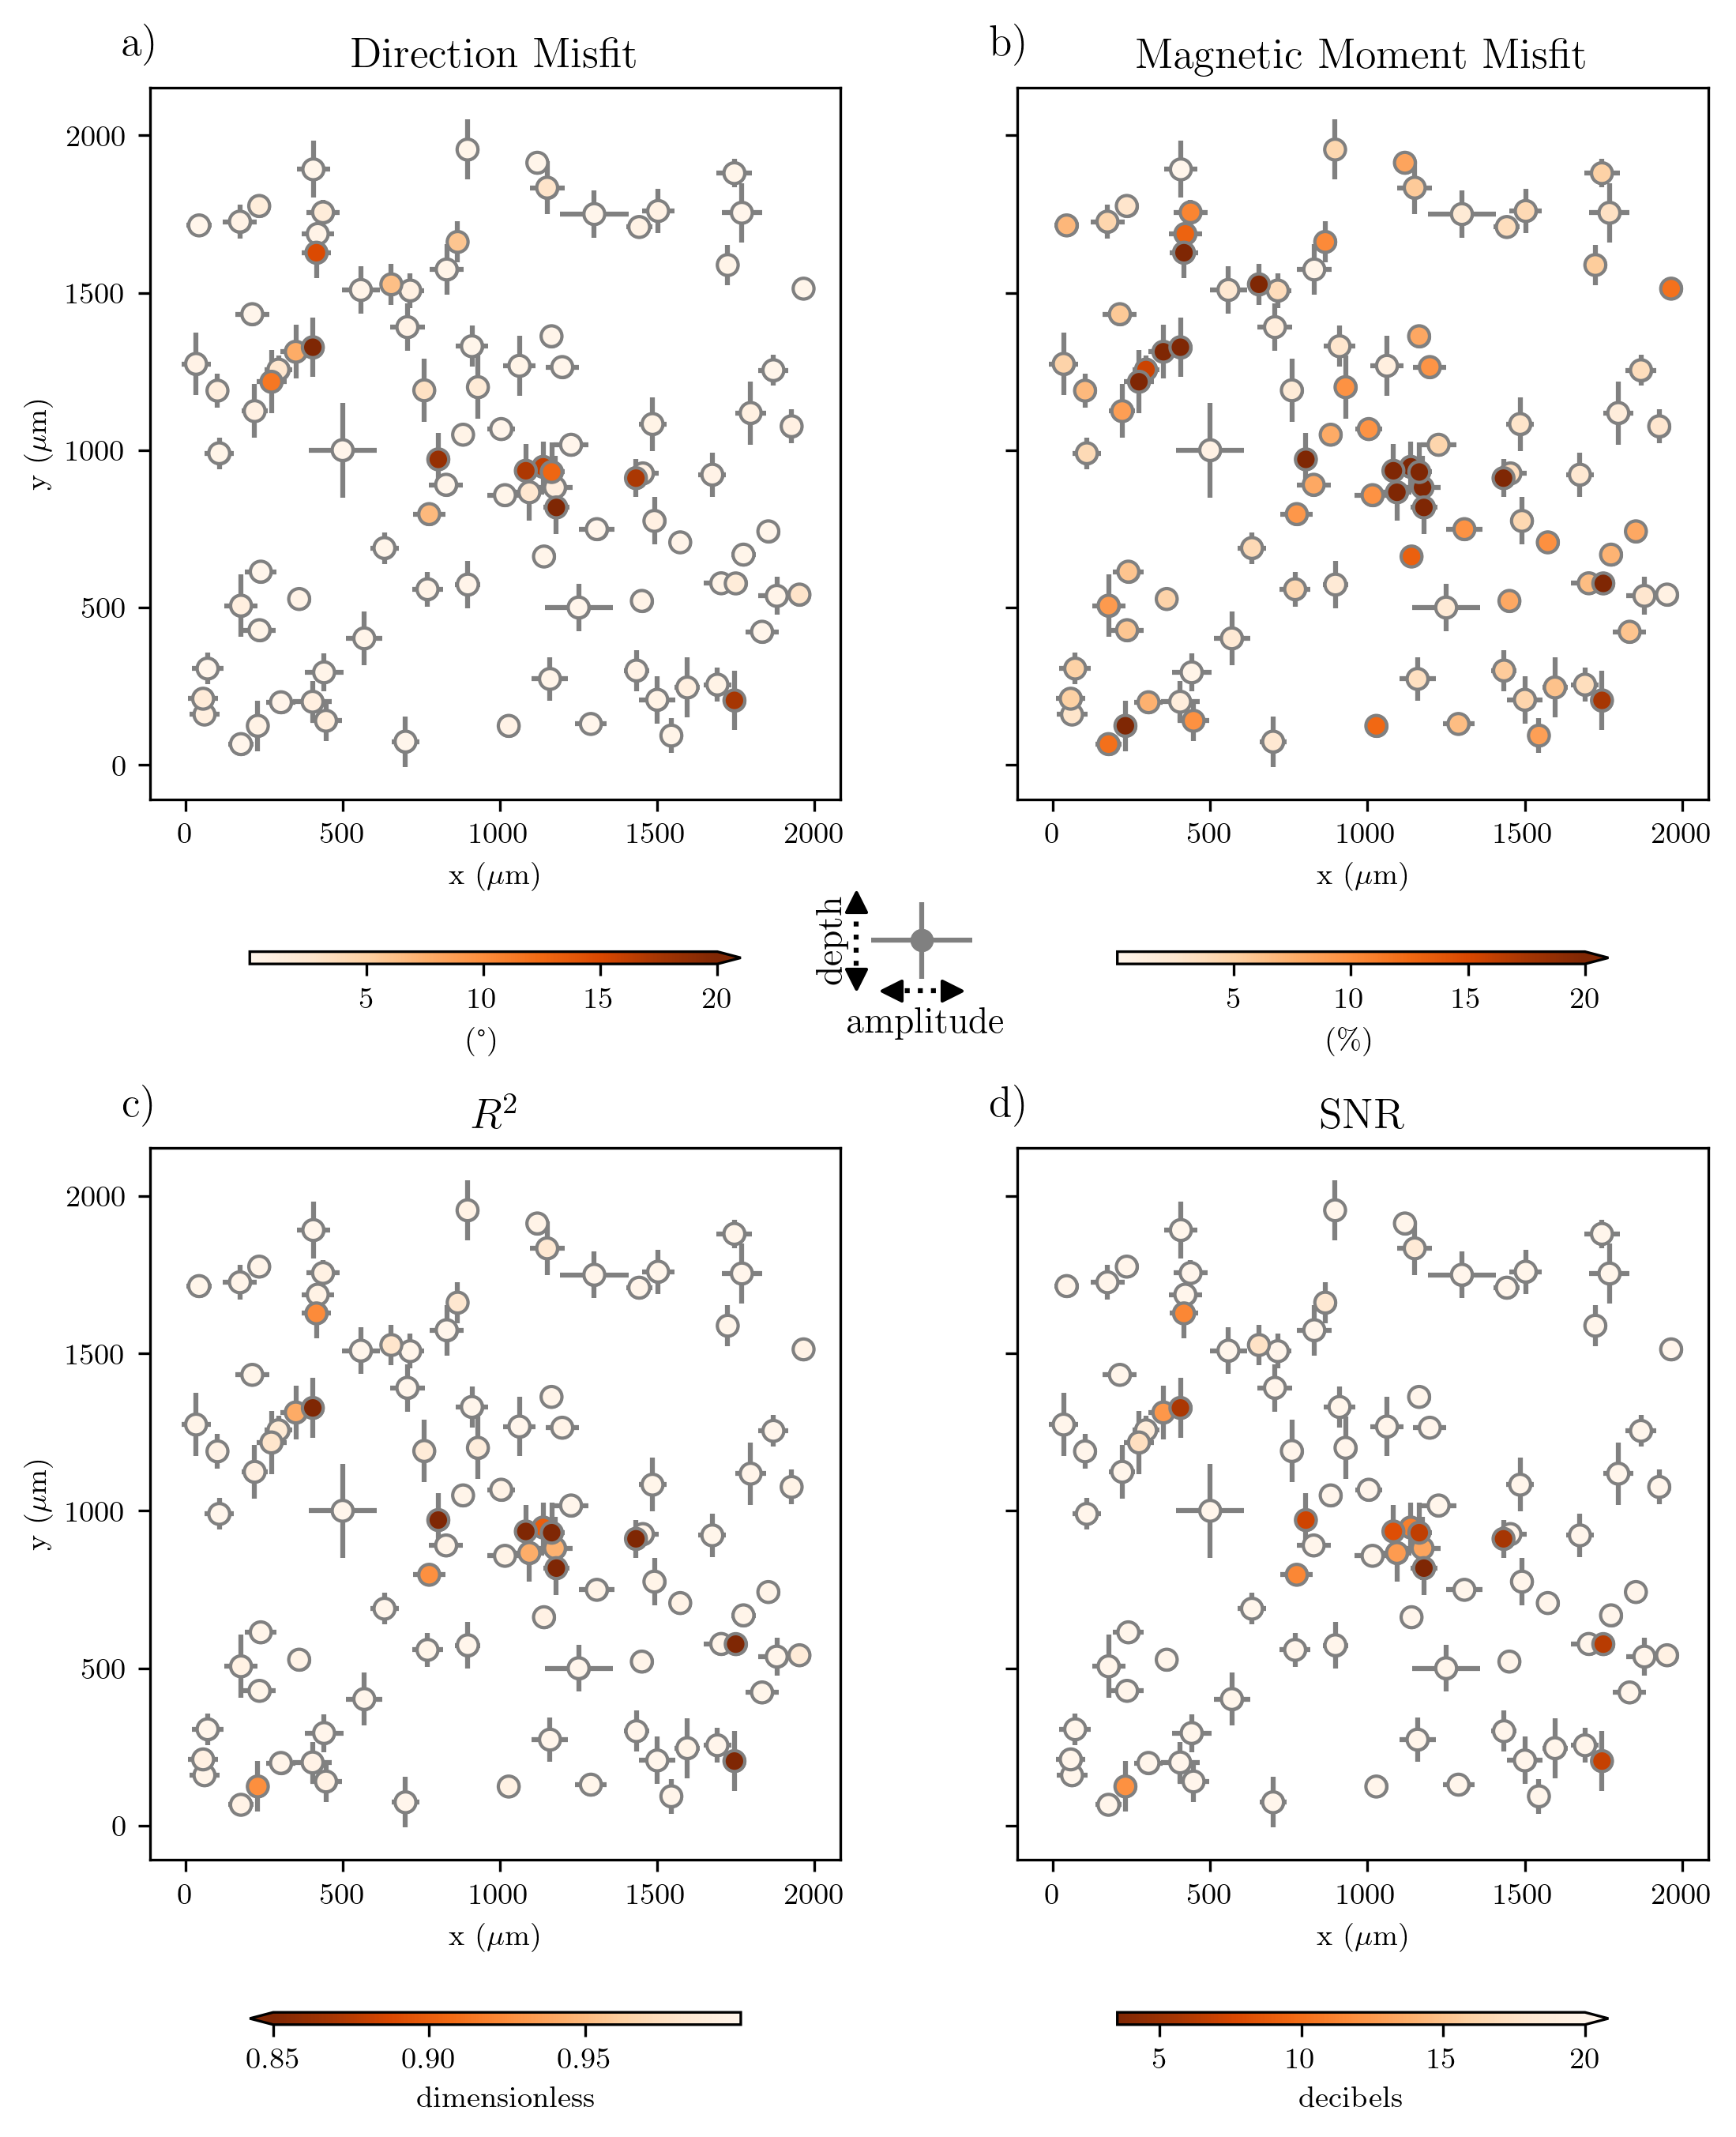
\includegraphics[width=0.75\linewidth]{figures/complex-synthetic-comparison.png}
\caption{
The validation of the result obtained with the inversion was calculated for each individual particle based on the error between the real parameters modeled and their respective recovered values, being (a) the direction and (b) intensity of the magnetic moment, in addition to the $R^2$ score (c) obtained by comparing the forward model and the actual data. The depth and radius of the magnetic sources are also important factors that influence the final result, therefore, these data are given in the form of cross plots, with the vertical bar represented by the depth (1 - 20 $\mu m$) and the horizontal bar by the dipole moment amplitude ($10^{-12}$ to $10^{-14}$ $Am^2$).
}
\label{complex-synthetic-comparison}
\end{figure}

The spatial resolution of the inversion results is one of the key advantages of magnetic microscopy over the classic techniques of paleomagnetism.
Therefore, we present the inversion results spatially so that we can evaluate any patterns in their distribution.
Figure~\ref{complex-synthetic-comparison} shows the spatial locations of the 99 sources that were identified and the differences between the estimated dipole moments and the true values.
The depth and dipole moment amplitude of each source are represented by horizontal and vertical bars, respectively.
These two variables are useful proxies for the strength and spatial extent of the signal of each source,
which can tell us about the limitations in strengths and sizes of the source signal that the technique is able to correctly invert.
Figure~\ref{complex-synthetic-comparison}a shows the absolute value of the angular difference between the true and the estimated dipole moment vectors.
Figure~\ref{complex-synthetic-comparison}b shows the percentage difference between the true and estimated dipole moment magnitudes ($|100 \left( m_{true} - m_{estimated}\right) ~/~ m_{true}|$).
Figure~\ref{complex-synthetic-comparison}c shows the $R^2$ coefficient (Equation~\ref{eq_r2}), which is equivalent to the non-dipolarity parameter of \citet{Fu2020} and represents how well the dipolar model is able to explain the observed data of each source.
Figure~\ref{complex-synthetic-comparison}d shows the SNR (Equation~\ref{eq_snr}), which expresses the power of the observed data over that of the inversion residuals.
High SNR values correspond to small inversion residuals which indicate that a dipolar model was able to explain the observed data.
Consequently, the variation of SNR values is similar to that of the $R^2$ coefficient.
Figure~\ref{complex-synthetic-comparison} shows that large errors in the estimated dipole moment direction are associated with low values of $R^2$ and SNR.
Conversely, the correlation between errors in dipole moment magnititude and $R^2$ and SNR is less pronounced, with some poor magnitude estimates being associated with $R^2$ and SNR indicating a good fit of the dipolar model.
It is also noticeable that the majority of cases where the dipole moment direction error is large are associated with deep and low-amplitude sources that are close to shallower or higher-amplitude sources.
These results indicated that $R^2$ and SNR can be used as selection criteria to discard sources with likely high errors in the estimated dipole moment.

\begin{figure}[tb!]
\centering
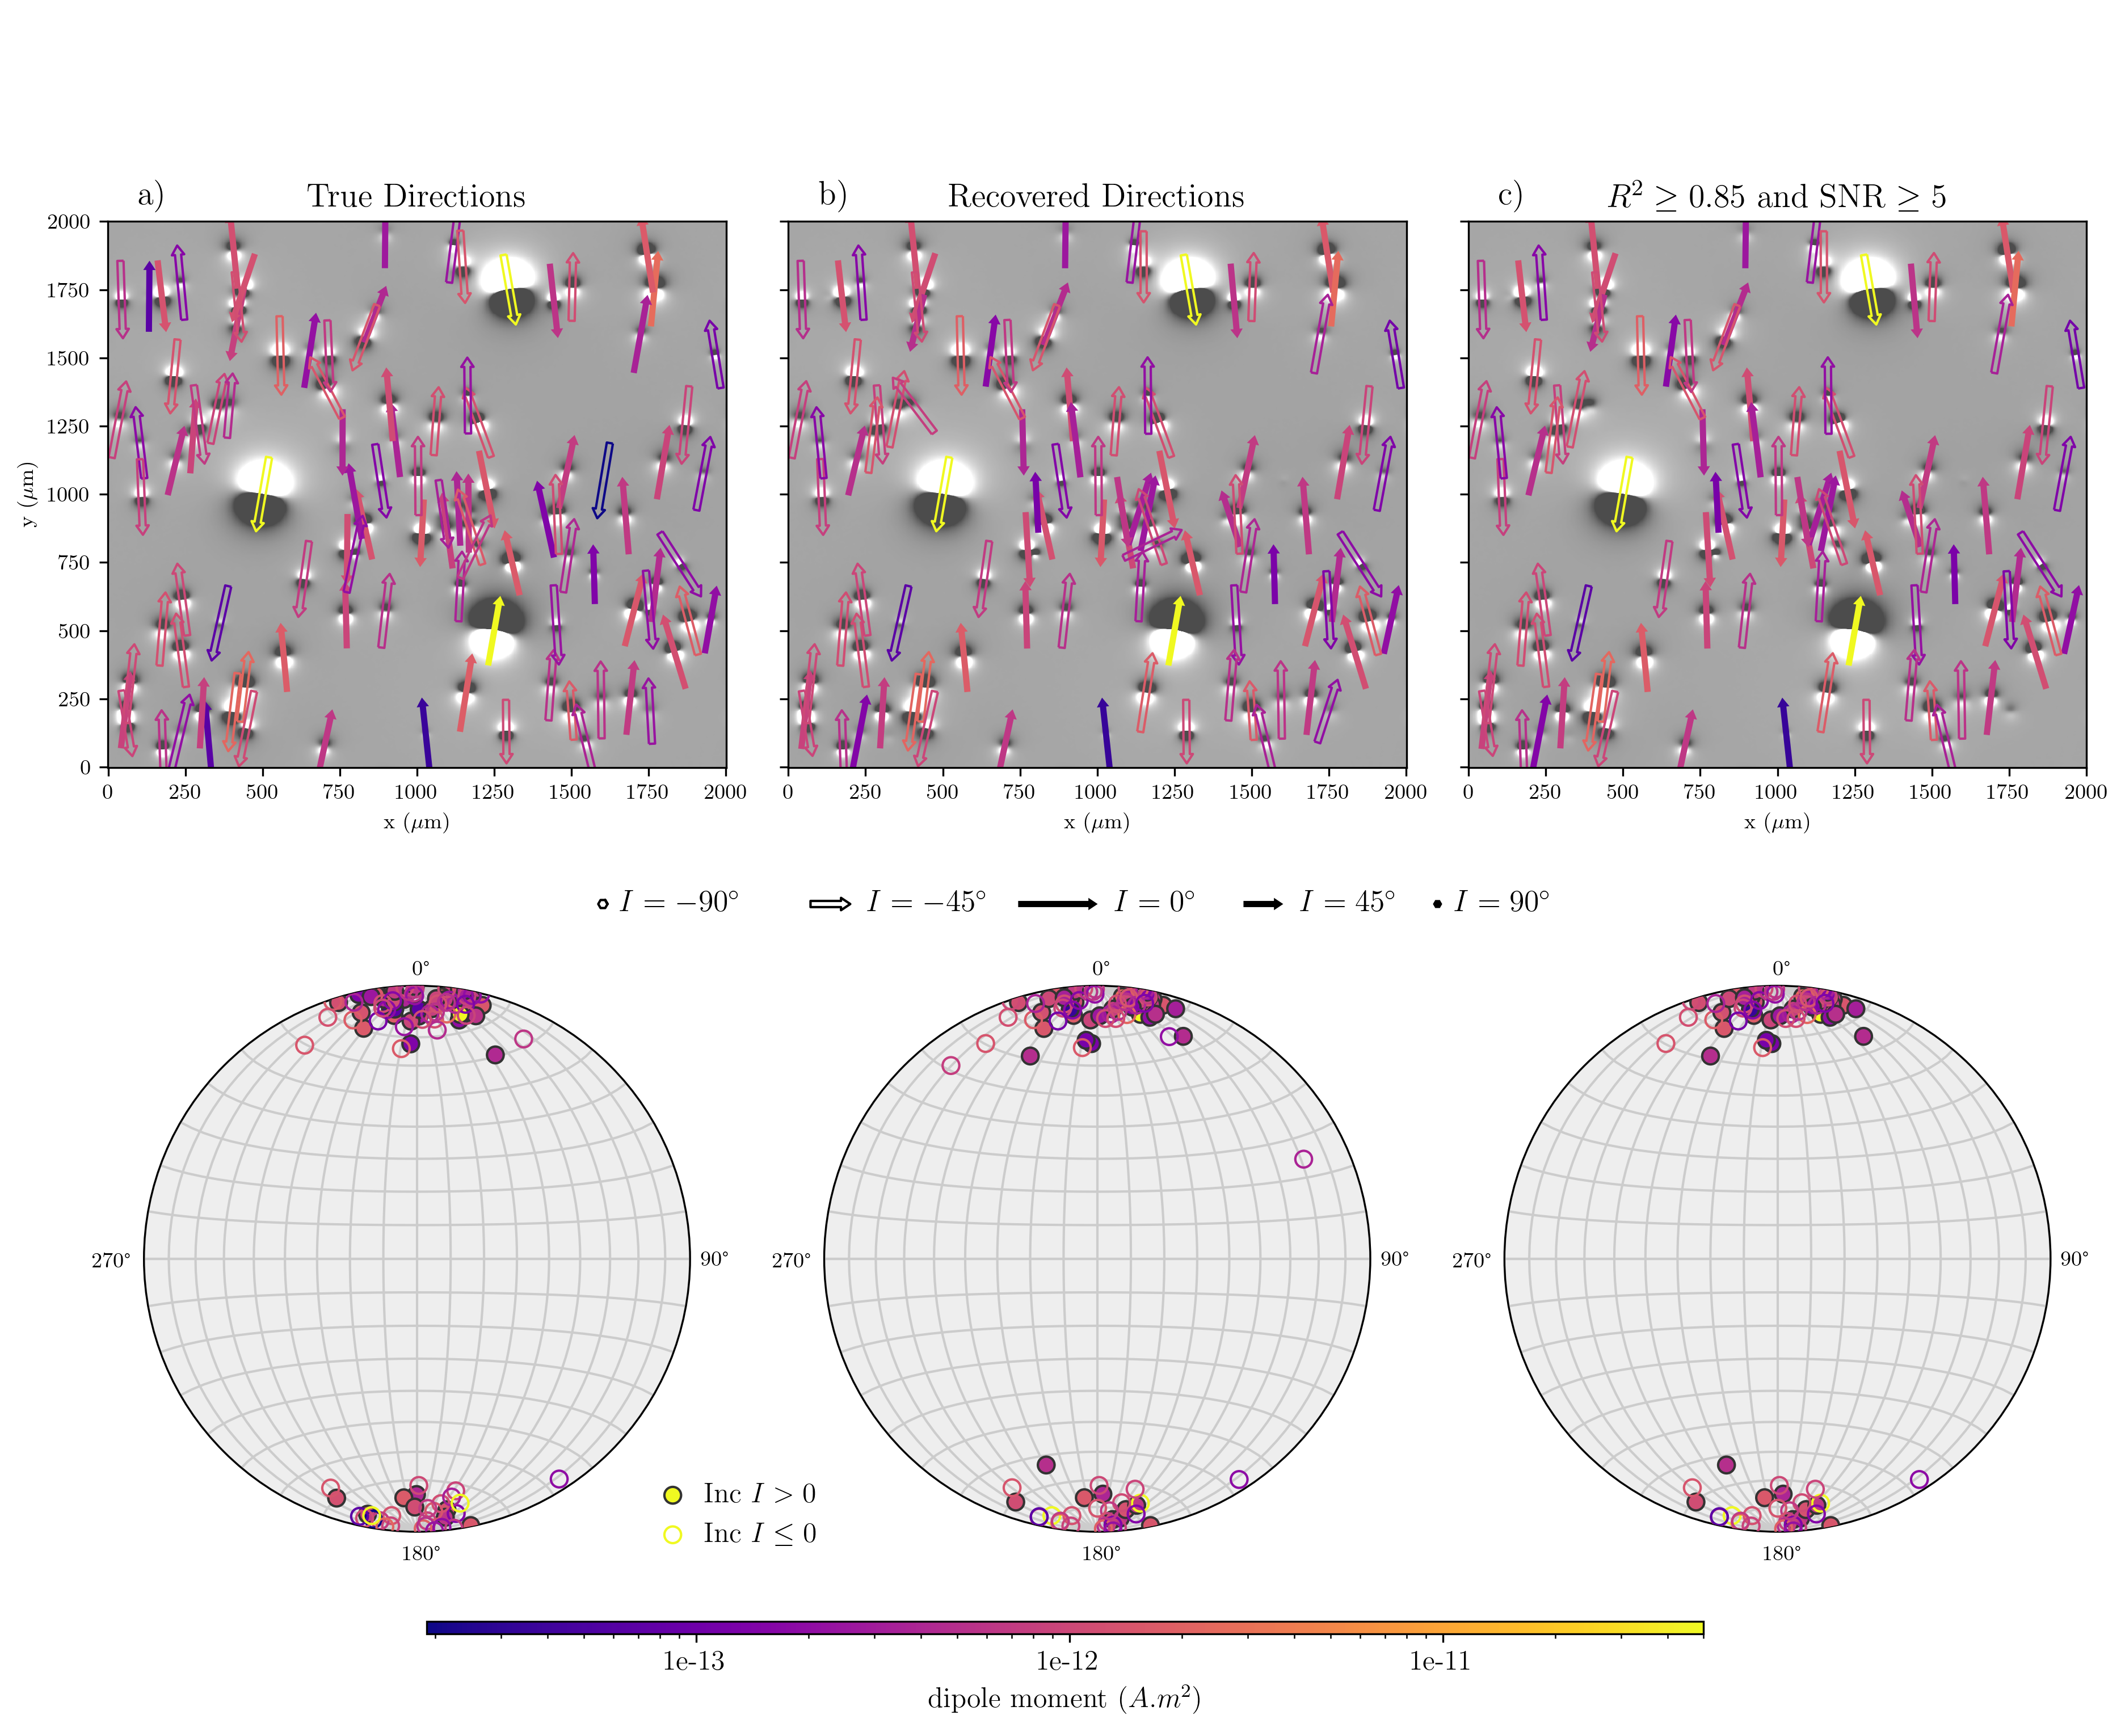
\includegraphics[width=1\linewidth]{figures/complex-synthetic-stereograms.png}
\caption{ Comparison of true and estimated dipole magnetic moments and directions for the complex synthetic sample.
a) Simulation of a thin section of rock with 103 particles uniformly magnetized (dipolar sources) by two different induced fields. The average directions of the induced fields are $D=\ang{0}$ and $I=\ang{0}$ and $D=\ang{180}$ and $I=\ang{0}$, yielding two stable directions. b) All estimated vector directions of the identified sources ($M=99$). c) The Filtering criteria used to select the magnetic directions of the sources with the best fitting ($M=96$), determined by the coefficient of determination ($R^2 \geq 0.85$) and signal-to-noise ratio ($\text{SNR} \geq 5$).
}
\label{complex-synthetic-stereograms}
\end{figure}

Figure~\ref{complex-synthetic-stereograms} shows stereograms with the directions generated by the modeled (Figure~\ref{complex-synthetic-stereograms}a) and the estimated vectors (Figure~\ref{complex-synthetic-stereograms}b) for each source. The distribution of the estimated directions is coincident with the true directions aside from a few sources, the same ones with the higher values of direction misfit (Figure~\ref{complex-synthetic-comparison}a) which is probably associated with the mutual interference of sources close to each other or within the same window. When filtered to include only data with R\textsuperscript{2} \textgreater 0.85 and SNR \textgreater 5 the obtained direction distribution is closer to the true distribution (Figure~\ref{complex-synthetic-stereograms}c).


%%%%%%%%%%%%%%%%%%%%%%%%%%%%%%%%%%%%%%%%%%%%%%%%%%%%%%%%%%%%%%%%%%%%%%%%%%%%%%%
\section{Application to real data}

To test whether the proposed method would be able to determine the
magnetization directions and the magnetic moment of particles in natural
samples, we selected a previously studied carbonate stalagmite sample from the
Wintimdouine cave in the Agadir region (Morocco) \citep{Ait2019Hydro}. This
speleothem contains both magnetite and hematite as the main carriers of
magnetic remanence, as attested by thermomagnetic curves with temperature
decays at {\textasciitilde}580 °C and {\textasciitilde}680 °C, and bimodal
curves of isothermal remanent magnetization (IRM) acquisition \citep{carmo2019speleothem}.

In order to provide two distinct directions associated with the different
magnetic mineral types in this sample, we applied two IRM pulse fields of 2.7 T
and 0.3 T, respectively toward the +Y and -Y directions. In this way, the high
coercivity grains (hematite) would point towards +Y and the low coercivity ones
(magnetite) would align in the -Y direction.

After remanence acquisition, we performed a magnetic map with the Quantum
Diamond Microscope (QDM) at Harvard University over a sample section of
approximately $\qty{1410}{\um} \times \qty{2256}{\um}$ (Figure~\ref{real-data}a) with a grid
spacing of \qty{2.35}{\um} and a sensor-sample distance of approximately \qty{5}{\um}, totaling
576,000 data points. The QDM is housed in a shielded room, in
order to avoid the influence of the Earth's magnetic field while the data were taken in projected magnetic microscopy (PMM) mode and converted to the vertical component of magnetic field ($b_z$) using a spectral approach \citep{Lima2009, Fu2020,
Glenn2017}. We applied a bias field of \qty{0.9}{\milli\tesla} during the measurement, which was periodically reversed to result in an effective background field of $< \qty{1}{\micro\tesla}$.  After applying the magnetic anomaly detection algorithm (Figure~\ref{real-data}b-e), it was
possible to determine the windows for 75 potential sources, as shown in Figure~\ref{real-data}e.

\begin{figure}[tb!]
\centering
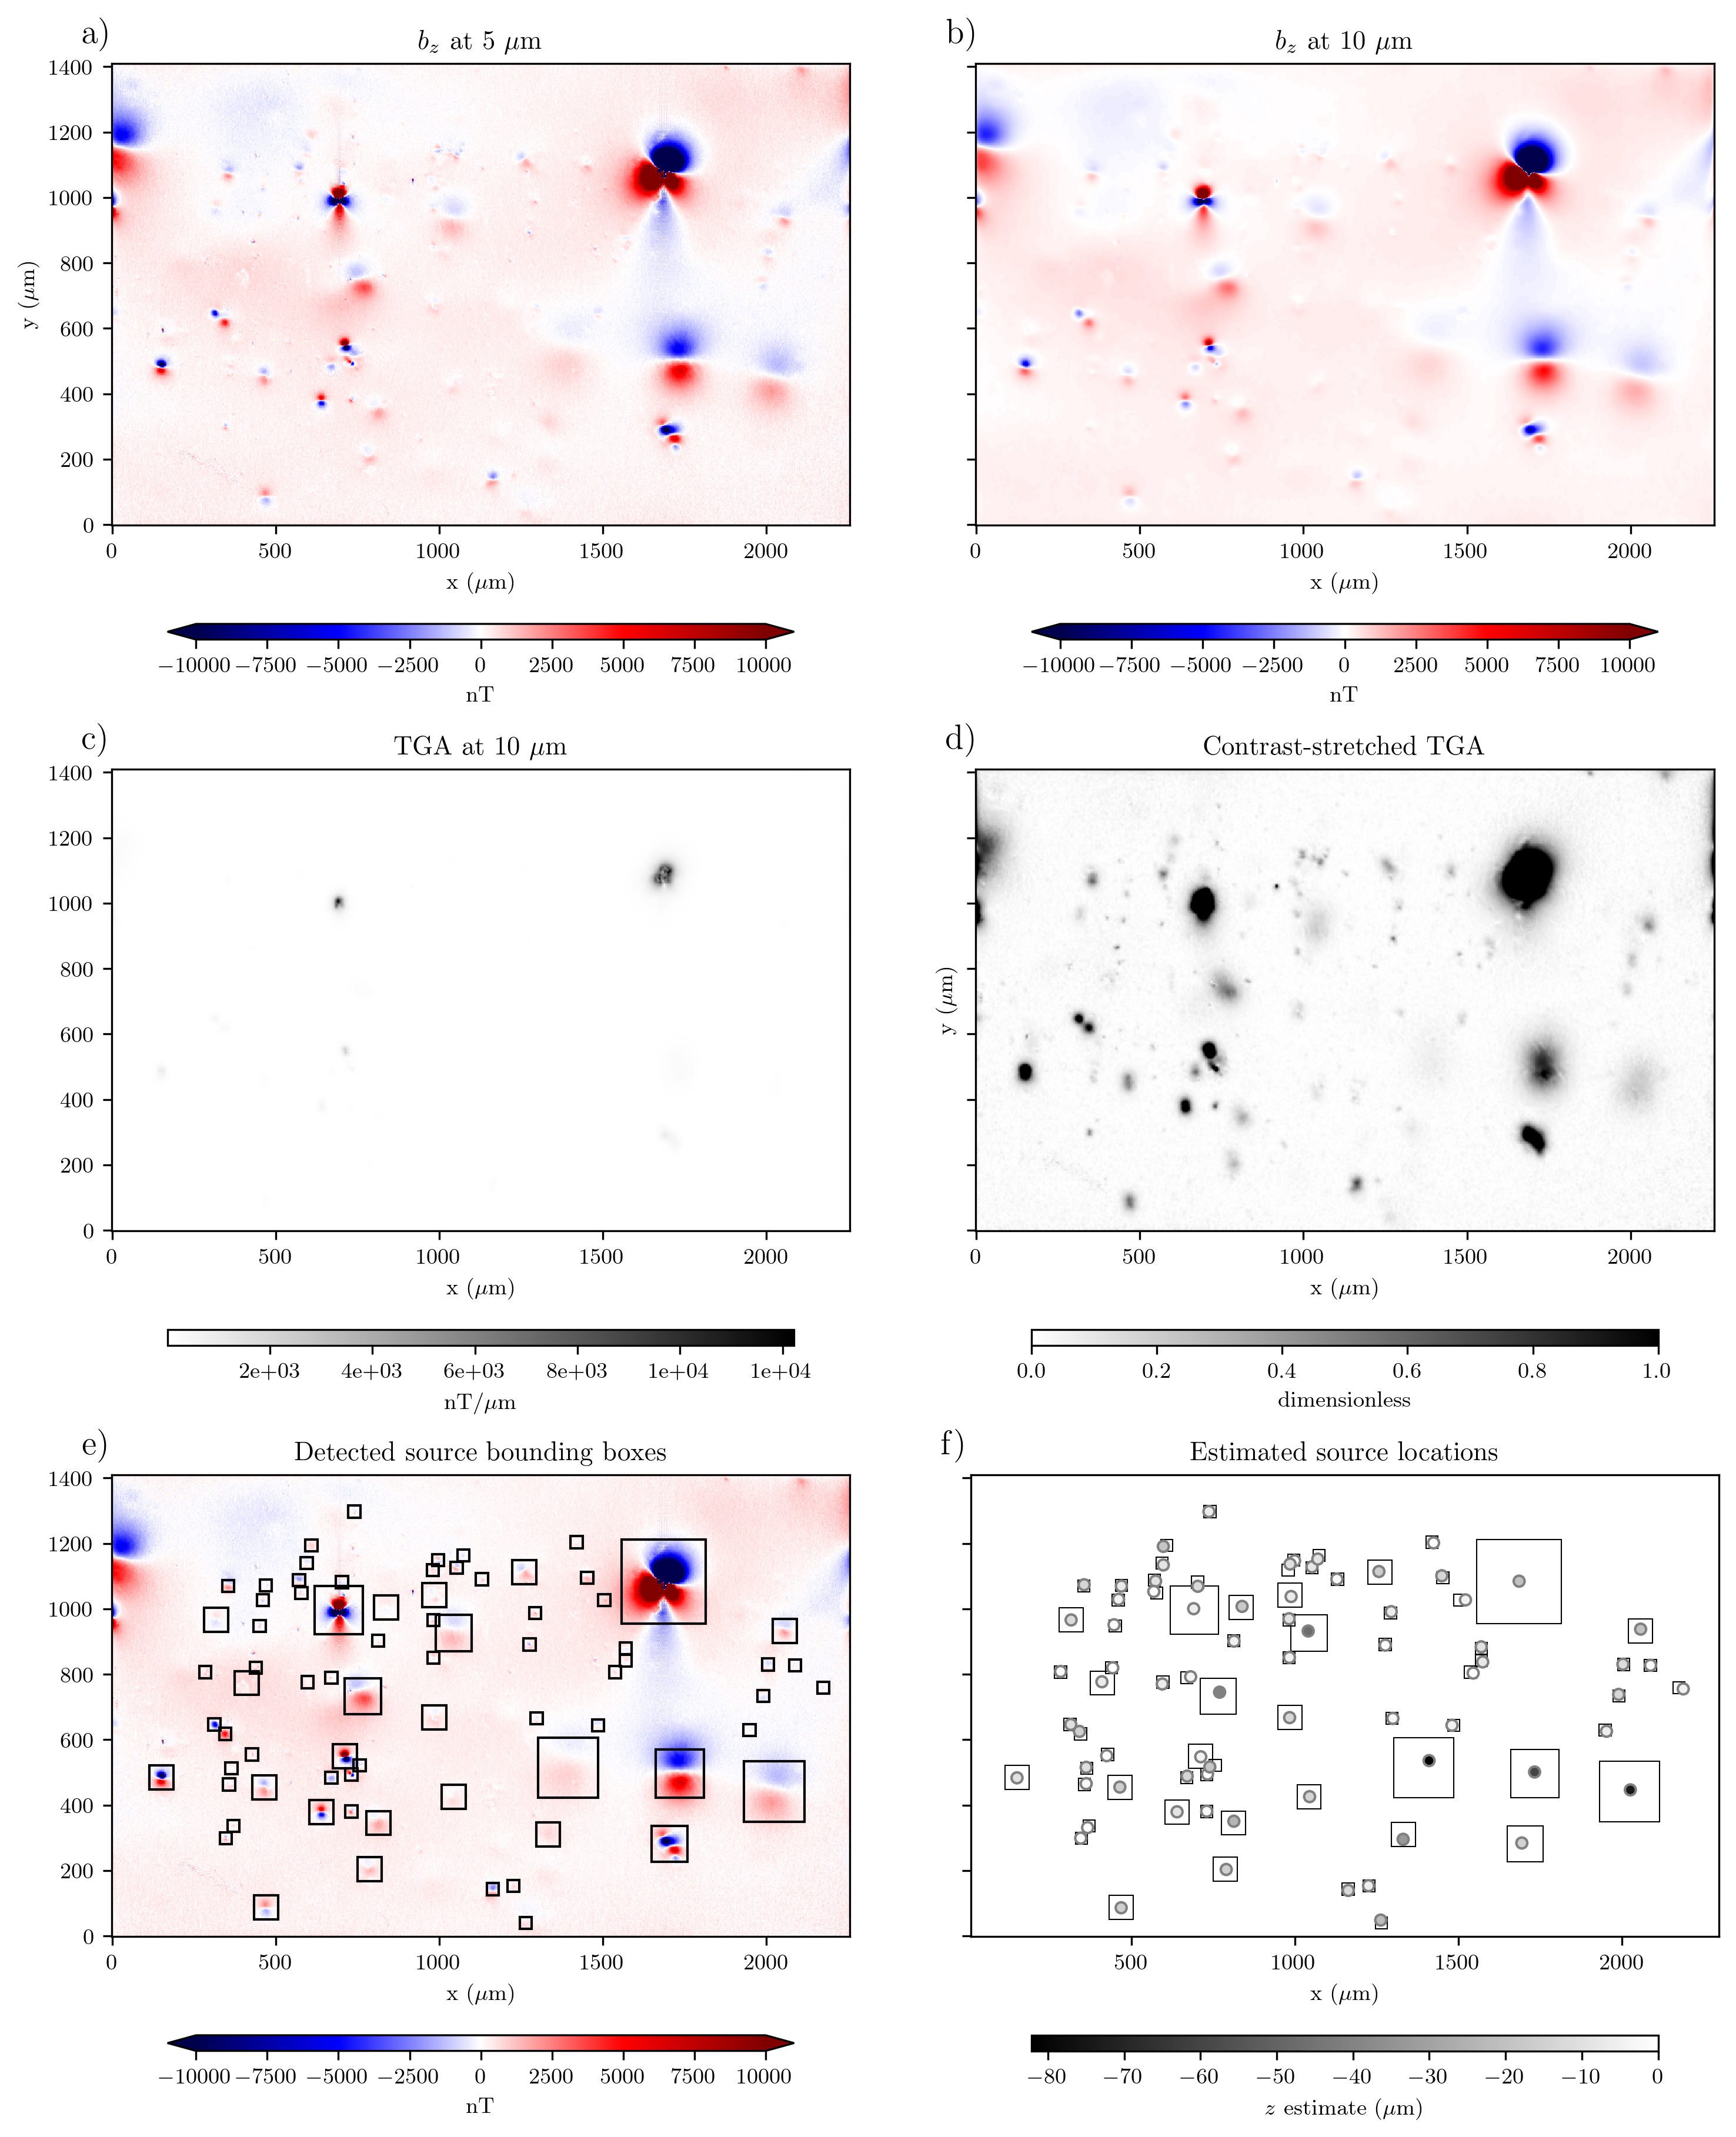
\includegraphics[width=1\linewidth]{figures/real-data.png}
\caption{Real data and the various processing steps performed prior to the dipole moment inversion.
    a) The real sample vertical component magnetic data $b_z$ observations at
    $z = \qty{5}{\um}$.
    b) Anomaly map after the upward-continued data to $z = \qty{10}{\um}$ to attenuated long and short-wavelength noise.
    c) The total gradient amplitude (TGA) calculated from the
    upward-continued data.
    d) The contrast-stretched TGA.
    e) The detected source bounding boxes (black squares) that correctly
    encapsulate the main signal of the sources.
    f) The estimated source locations (colored circles) from Euler
    Deconvolution of the upward-continued data inside each bounding box.
    The color represents the estimated $z$ coordinates.
  }
\label{real-data}
\end{figure}

After applying the ED algorithm, we performed the inversion of the magnetic moment for each of the 75 windows selected previously. In order to reduce considerably the computation time, the inversions were done within each data window, instead of solving all sources parameters at the same time. We obtained the magnetic moment and the direction for all 75 magnetic grains (Figure~\ref{real-data-stereograms}a). Then, we calculated the residuals of the inversions in each window and subsequently the coefficient of determination $R^2$ and signal-to-noise ratio (SNR), which were parameters used as filters for the best directions obtained. We considered a good fit to be achieved when $R^2$ was greater or equal to 0.85 and SNR was greater than 5. An $R^2$ value of 0.85 indicates that \qty{85}{\percent} of the measured magnetic data is explained by the predicted dipole model, which is equivalent to the dipolarity test approach \citep{Fu2020}. On the other hand, an SNR of 5 means that the dipolar signal is 5 times greater than the residual noise. By using these criteria, we ensured that the fit was sufficiently accurate and the dipole model provided a reliable approximation of the original magnetic data. About 46 identified sources passed these criteria. This filtering technique removed the poorly fit predicted models as well as the ones too corrupted with noise, showing more clearly the expected directional clusters of hematite and magnetite crystals (Figure~\ref{real-data-stereograms}b). Notably, it is confirmed that the sample has both magnetic minerals, but by the expected directions we can also stipulate that the magnetite grains outnumber the hematite ones.

\begin{figure}[tb!]
\centering
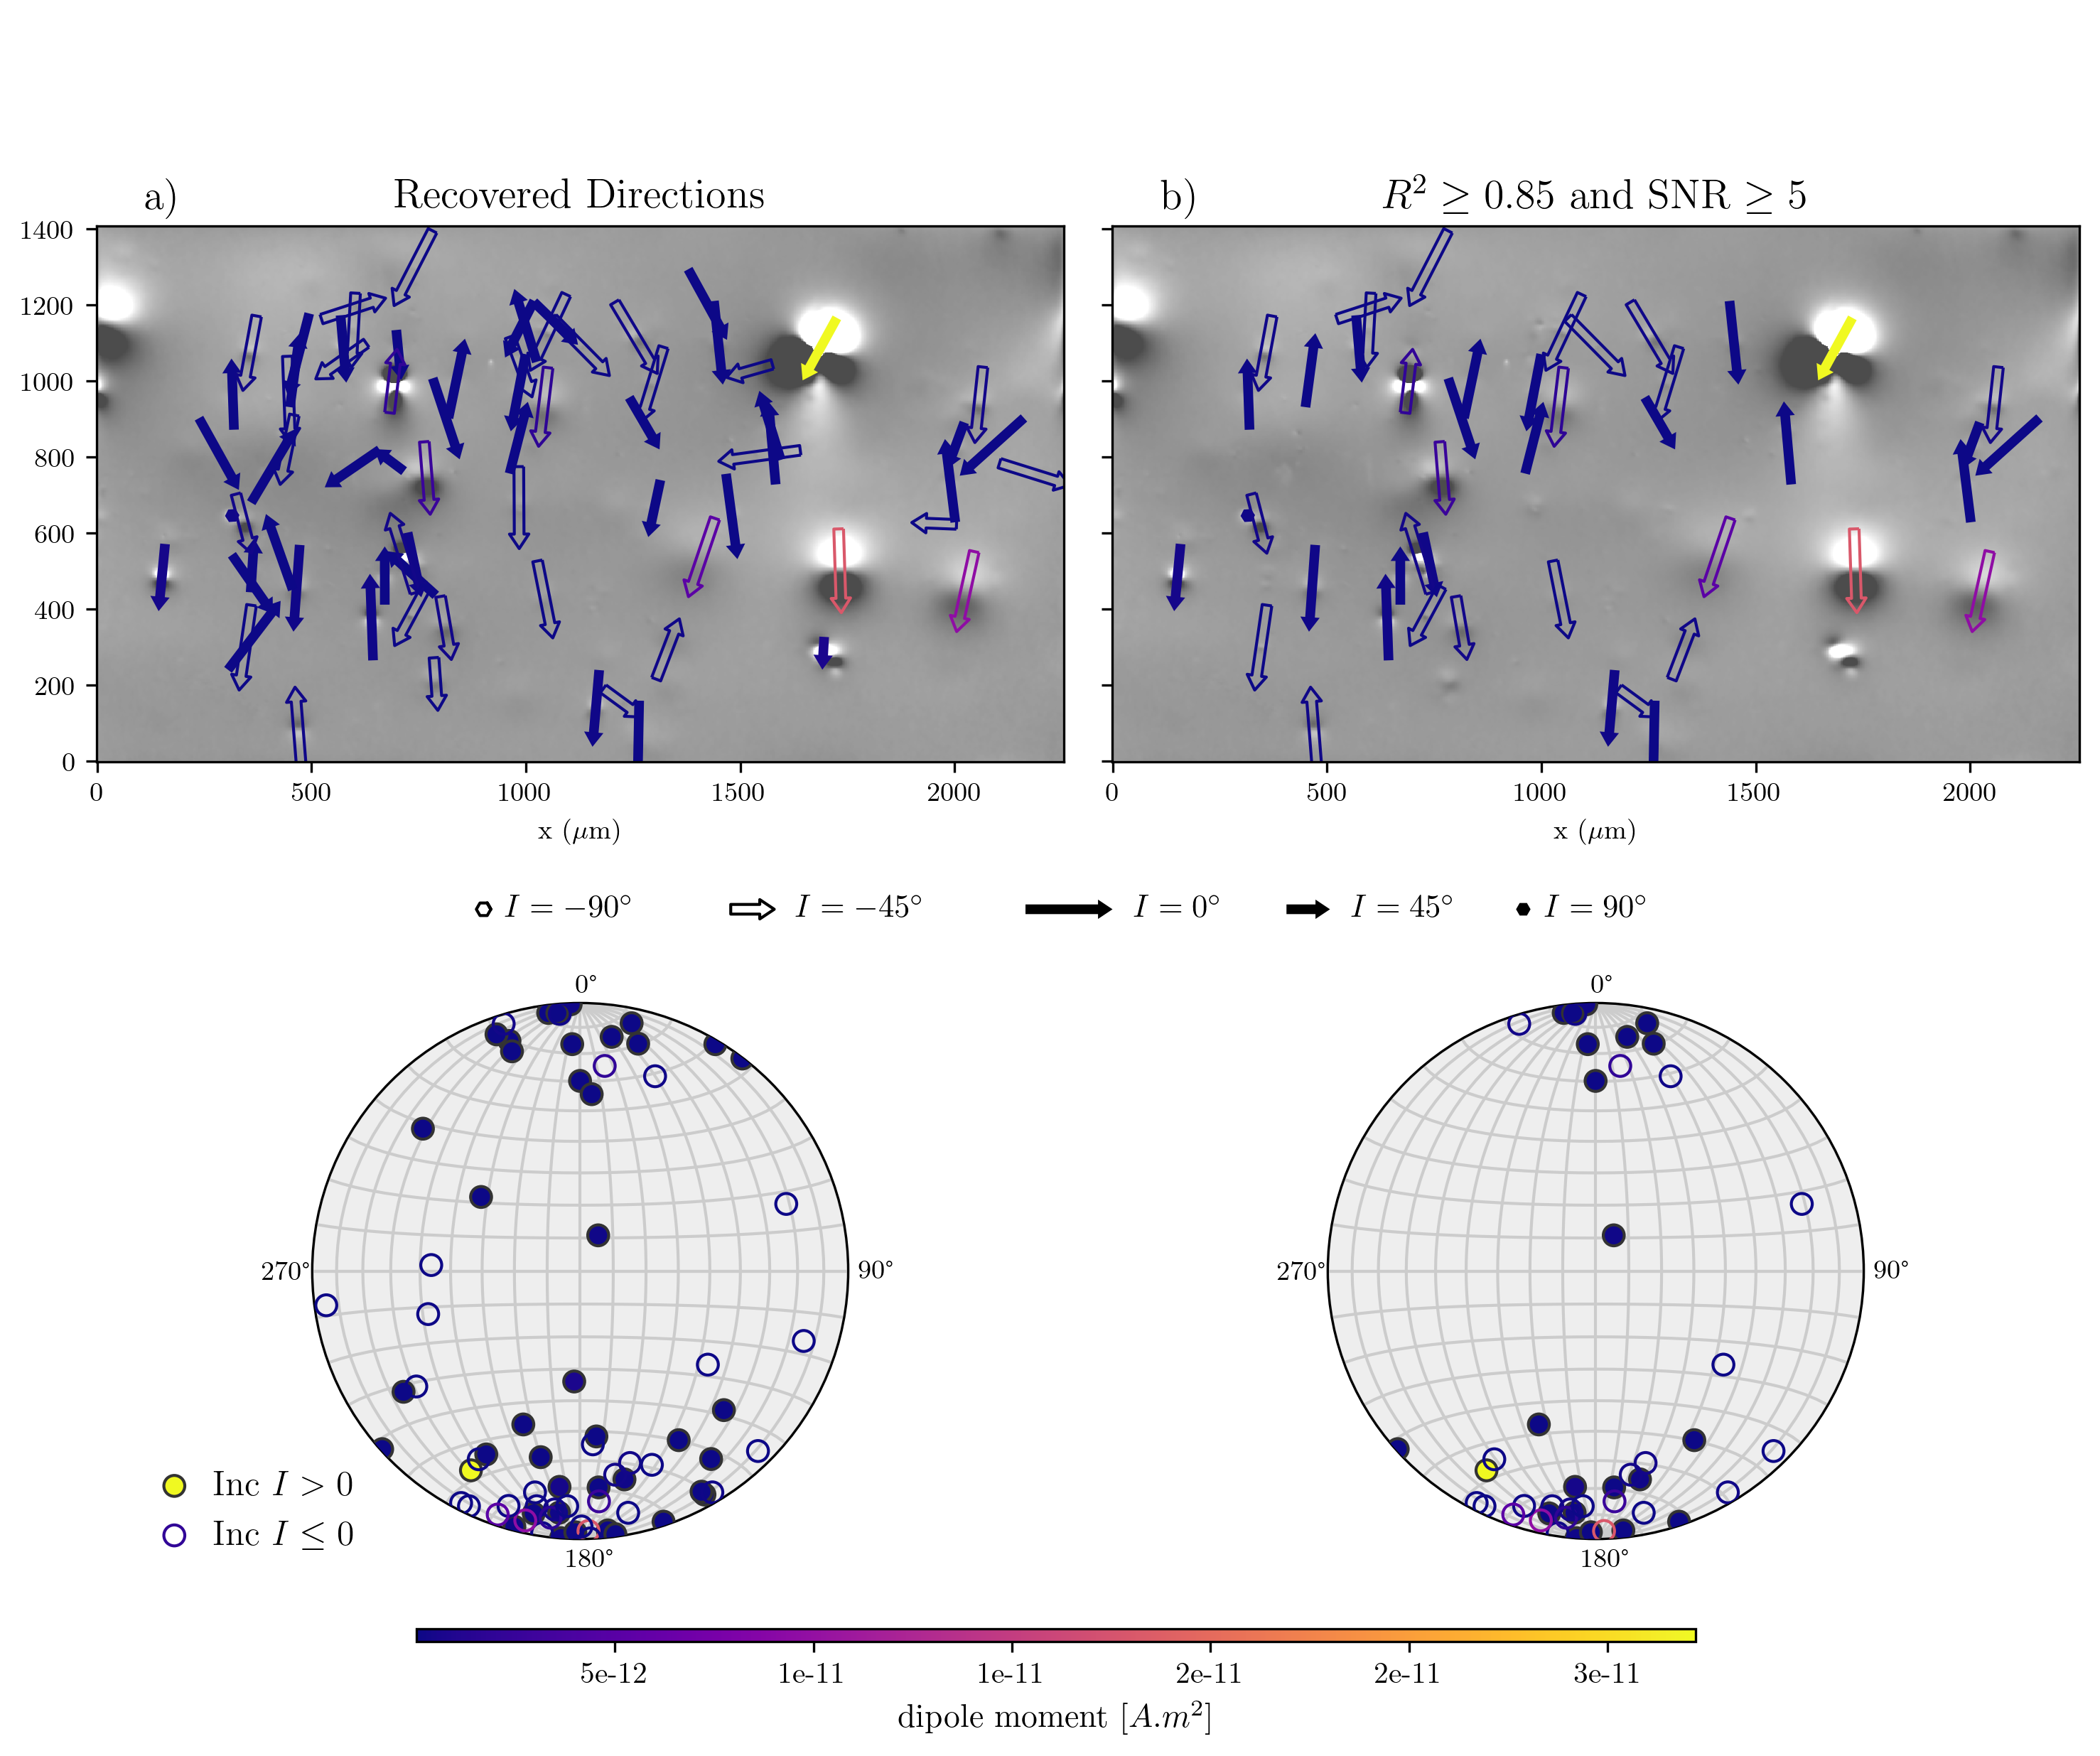
\includegraphics[width=1\linewidth]{figures/real-data-stereograms.png}
\caption{
Comparison of the estimated dipole magnetic moments and directions for the real data sample.
a) All estimated directions without filtering ($M=75$). b) Estimated directions filtered ($M=46$) by the coefficient of determination ($\geq 0.85$) and SNR ($\geq 5$), which shows two clusters of direction located on each pole of the stereogram.
}
\label{real-data-stereograms}
\end{figure}

%%%%%%%%%%%%%%%%%%%%%%%%%%%%%%%%%%%%%%%%%%%%%%%%%%%%%%%%%%%%%%%%%%%%%%%%%%%%%%%
\section{Discussion}

\subsection{Prior information and uniqueness of solutions}

Working with potential field data might be very tricky once there is too much ambiguity involved during data modeling, thus to obtain unique and reliable results from data inversion it is necessary to provide as much prior information as possible.
One way to circumvent the ambiguity is to incorporate prior information about the subsurface structure, such as the positioning of a known source of magnetization.
Magnetic field measurements are more sensitive to changes in magnetization near the source that is causing the anomaly.
When the position of the source is known, it constrains the model to be as consistent as possible with the observed data, hence increasing the likelihood of obtaining unique solutions.
\citet{Oliveira2015Estimation} proved that the magnetization directions (Dec and Inc) recovered by the least squares estimator are sensitive to great variations in the horizontal coordinates of the center of the magnetic sources, but are practically insensitive to variations in depth.
Thus, they consider the ED method as an adequate technique to estimate the central positions that will be used as prior information for inversion.
This occurs mainly because, when well performed, the recovery of the source's horizontal coordinates is considerably accurate, while the vertical coordinate can undergo greater variation even though it still provides satisfactory results \citep{Silva20033D, Melo2013}.
This remark is also better observed in our simple synthetic sample where the estimated horizontal positions slightly deviate from the true values, which implies small misfit values in the recovered magnetic directions.
Although the estimated magnetic moment for the said sample is satisfactory, this magnetic parameter is more affected by the variations in the depth of the source, which is probably caused by ambiguities.
In summary, in order to estimate all magnetic parameters as precisely as possible the ED must be executed within a data window containing the lowest amount possible of noise since that high-frequency noise sensibility is one of the ED's main limitations.

\subsection{A critical examination of the source detection}

Since the pioneering work of \cite{Egli2000}, many methodologies were proposed for solving the inverse problem o micromagnetic data, and for the purpose of comparison we separate them into two categories based on the main estimated parameter by the inversion procedure.
In the first type of approach, the main goal is usually to estimate average magnetization by inverting the whole sample superficial magnetization data commonly by means of unidirectional problem, uniform directions with non-negative variable dipole moments \citep[e.g.,][]{Weiss2007}, including performance enhancement in the spatial domain \citep[e.g.,][]{Myre2019} or frequency domain  \citep[e.g.,][]{Lima2013}.
This methodology can be used to remarkably estimate the average magnetic direction and the total moment direction with the assumption that the particles were all magnetized in the direction of the same induced field \citep[sIRM and/or NRM in basalts,][]{Weiss2007}.
However, this assumption is not always true when dealing with complex samples (i.e., more than one stable direction), which leads to the same drawbacks as the classic paleomagnetic measurements using bulk samples.
The second type of approach has the goal of finding the individual source magnetic properties, which can be done by either inverting the dipole moment of a single source within a cropped section of an upward continued anomaly map \citep[e.g.,][]{Lima2016, Fu2020} or by the insertion of additional information of the sources’ shape, such as micro-computed tomography (microCT) \citep[e.g.,][]{Fabian2019, DeGroot2018, DeGroot2021}.
The latter further allows unique estimation of magnetic moment configuration of even higher orders components through spherical harmonics expansion constrained by micromagnetic models \citep[e.g.,][]{CortesOrtuno2021, CortesOrtuno2022}.
Such outstanding techniques come with some troubles of having to mechanically select the data for inversion or dealing with the weaknesses of the additional method used.
The MicroCT, for example, is a popular non-destructive technique for high-resolution imaging of the material internal structures, and yet, it is accompanied by some limitations when it comes to paleomagnetic studies: firstly, the technique has a spatial resolution on the order of micrometers, which is not sufficient to directly image the fined grained single-domain magnetite \citep{DeGroot2018}.
The microCT also struggles to discern ferromagnetic (\textit{l.s.}) from non-magnetic/antiferromagnetic minerals, as pointed out by \cite{DeGroot2021}, since they usually have similar densities and therefore similar X-ray attenuation \citep{Cnudde2013}.
In any case, the major limitation of microCT lies in the trade-off between the resolution and the sample size, requiring small sample volumes to achieve higher resolutions causing the technique to be too time-consuming.

Our proposed methodology has the goal of finding each individual source’s dipole moment components without the trouble of mechanically selecting cropped data or needing any type of additional information.
However, to better examine its advantages and disadvantages we first need to point out the strengths and weaknesses of the technique used in the detection of sources, the Laplacian of Gaussian (LoG) kernel \citep{Marr1980}.
The LoG is a computer imaging technique that is able to identify regions where the intensity changes abruptly by convolving the image with the LoG filter, and is the result of the combination of the Gaussian blur and Laplacian filter \citep{gonzalez2018}.
The Laplacian filter is able to highlight the regions where the intensity changes rapidly.
On the other hand, the Gaussian blur is a smoothing filter for high-frequency noise, which reduces the likelihood to generate artifacts.
Hence, the result of this LoG operation can identify blobs as regions above a certain threshold, this threshold crossing determines what are brighter spots (local maxima) surrounded by a darker background.
It is also scale-invariant by detecting blobs of different sizes and intensities, a feature achieved by varying the sizes of the Gaussian filter.
The advantages of the methodology are (i) high-accuracy blob detection; (ii) scale-invariant for images with different intensities/sizes of objects; while also being (iii) robust to the presence of noise due to the Gaussian smoothing filter.
While the main drawbacks of the LoG blob algorithms are: (i) being computationally expensive/time-consuming when dealing with larger images and (ii) the requirement of parameter adjustments, such as the threshold and the kernel sizes.

The total gradient anomaly (TGA) might be considered the ideal image to be used as input for the LoG blob detection algorithm for potential field studies (micro and/or macroscale).
The TGA highlights the subsurface sources by generating a map of positive magnetic anomalies concentrated within their edges.
This technique is widely used in aeromagnetic surveys to determine the boundaries of sources by calculating the magnetic gradient in all Cartesian directions and displaying those regions where the gradient has maximum values, which is a local maxima distribution.
Hence. The application for micromagnetic measurements comes with all the advantages and drawbacks previously mentioned because is highly dependent on the selection of a good data window.
Nonetheless, the windows generated isolate the main magnetic signal’s region of each source.
This guarantees that our thresholding approach (see section~\ref{dipole-reliability}), for both ED and dipolar inversion, is performed using the critical slice of the micromagnetic data, giving satisfactory parameters approximation and fast results as shown in the synthetic data.

The complex synthetic data allows better observation of the strengths and limitations of the windows approach.
The main strengths that can be mentioned are: (i) the applied technique not only detects most of the modeled sources but also (ii) most of the recovered magnetic parameters have considerably low errors, especially in the directions, usually less than 5° (Figure~\ref{complex-synthetic-comparison}a).
(iii) The magnetic moments obtained from well-individualized sources tend to not deviate much from the real values (Figure~\ref{complex-synthetic-comparison}b) when $R^2$ and SNR scores are considered high ($\geq 0.85$ and $\geq 5$, respectively) (Figure~\ref{complex-synthetic-comparison}c-d).
(iv) Shallow particles grouped in clusters are usually well individualized during window selection, as well as (v) some isolated particles that produce a weak magnetic signal.
The major limitations observed were: (i) the blob detection fails when there are sources too close, grouping them into the same window, thus causing an erroneous result both for Euler deconvolution and for the magnetic parameters.
(ii) The very same occurs when there is a source under another, in this case, the magnetic signal is the sum of both.
(iii) In clusters of larger and/or deeper particles, although the method individualizes them well, the magnetic signal of the neighboring particles can considerably influence the result of the inversion, especially the estimated dipole moment (cluster in the Figure~\ref{complex-synthetic-comparison}b with the highest misfit values).
As expected, there is a direct relationship between the dipole intensity and depth with the observed errors.
It is clear from the error bars in Figure~\ref{complex-synthetic-comparison} that deep-seated sources and/or particles with small dipole moments generate worse results, essentially because they will produce weaker anomalous fields in the magnetic maps.
Note nonetheless, that even sources with small dipole moments when close to the surface are adequately modeled by our method, because of the trade-off between signal and noise for grains near the sensor.


\subsection{Reliability of dipole moment approximation}
\label{dipole-reliability}

Our approach relies in the premise of assuming the magnetic anomaly within
the data window is a response of a dipolar source.
The latter is true when working
with particle signals in the SD magnetic domain state since they are uniform magnetized particles with strong dipolar anomalies.
However, \cite{Nagy2017} reported that particles within the PSD domain can record the paleomagnetic field for longer (than SD ones) periods of time, being the stabler and also with strongly non-dipolar characteristics.
Therefore the application of the proposed algorithm to natural samples should fail for those PSD particles.
\cite{CortesOrtuno2022} give important insights about the matter, they showed that PSD state particles present more accurate inversion results when considering the non-dipole components for small sample-sensor distances (\textless 1 $\mu$m), but for larger sensor distances the dipole as approximations are remarkably accurate, as the higher-order moments decay rapidly with distance and therefore have less
influence on the particle's magnetic signal.
Thus, our approach can be considered reasonable for working with both particle SD and PSD states signals.
The latter happens mainly due to the sensor height being usually greater than 5 $\mu m$, considering a particle on the immediate surface of the sample the higher-order moments are already quite attenuated, thus circumventing the prominent problems described for non-dipolar components.

Despite the excellent signal-to-noise ratio that the SMM provided with the
proximity of the sensor to the sample, it is worth mentioning that the
measurement noise can still overshadow the responses of very weak/small, or
deep particles, generating unreliable inversion results.
Therefore, it is necessary to keep a check to determine if the inversion reached a satisfactory prediction, such as the coefficient of determination and the
signal-to-noise ratio suggested by \citep{CortesOrtuno2021}.

While the windows approach violates the fundamental theory of the inversion problem that  requires the sampled area to be finite and encapsulated by the inversion domain to ensure the uniqueness of results \citep{Baratchart2013,Lima2013}, our technique is similar to the  one reported by \cite{Weiss2007}.
The last-mentioned involves thresholding the long-distance interaction
of each dipole in the SMM data, which excludes the effect of other dipoles by setting their contribution to zero, resulting in a sparse matrix that permits faster calculations.
In contrast to this approach, we employ the TGA map to select the windows and isolate the area containing the main signal of the desired dipole, while the area out of the boundaries of the window is less sensitive to variation in magnetic parameters of this particular source, hence we exclude them from the inversion domain.
This technique allows us to obtain the 3D positioning and an approximation of the dipole moment components of hundreds of sources within a few seconds, while the inversion is fast the time bottleneck of our methodology is associated with the blob detection process.


%%%%%%%%%%%%%%%%%%%%%%%%%%%%%%%%%%%%%%%%%%%%%%%%%%%%%%%%%%%%%%%%%%%%%%%%%%%%%%%
\section{Conclusion}

We developed an efficient semi-automated method to determine the direction of magnetization of dipolar sources on a microscale, as well as the estimate of their magnetic moment.
Being ideal for a reinterpretation for the application of methods of paleomagnetic studies using thin sections of rock samples.
This would be an attempt to improve the quality of results obtained by isolating the responses of more reliable recorders of the Earth's geomagnetic field.

We also present a new, faster, and cleaner way to solve the Euler equation in determining the positioning of magnetic anomaly sources using a pre-selection of magnetic anomaly source windows based on the Laplacian of Gaussian applied to total gradient anomaly maps.
In this way, reducing the numerous solutions to just one data window per source.
After estimating the structural index ($n = 3$) by approximating the sources generating the magnetic anomaly to spheres/points, the Euler Deconvolution is performed, and the central position of each source is determined.
Due to the similarity with aeromagnetic data, this approach can also be extrapolated for macro-scale studies.

To recover magnetic direction and moment we only need to assume that the sources have their central positions known (so we apply Euler deconvolution) and that their magnetization is uniform.
This last premise aligns with the theory of magnetically stable particles SD, and by extension the PSD ones at a reasonable sensor-sample height, which is the basis of classical paleomagnetism.
Also, there is no need for any kind of prior knowledge other than the observed magnetic anomaly, and the structural index of the sources.
Therefore, this method can be quickly replicated in a data set of thin sections of rocks to obtain the distributions of magnetic directions of each source identified in the sample.

The test using a simple synthetic sample shows the great capability of the method by estimating not only the precise center positions but also retrieving the magnetization directions and intensity even under the considerable effect of high-frequency noise.
While the complex synthetic sample data allows observing the applicability of the method developed in real samples that are more complex with varied magnetization directions and intensity, in addition to also taking into account the high and low-frequency noise and sources with variable dipole moment intensities and depths.
The real sample data positively answered the question of the algorithm's ability to deal with thin sections of rocks.
But also, showed the acceptable capacity of retrieving different magnetization directions recorded by magnetic minerals with different coercivities and magnetic signal disparities even greater than predicted in the complex synthetic test.
We also assessed the quality of the fit between the predicted dipole model and the original magnetic data using two criteria: the coefficient of determination ($R^2$) and the signal-to-noise ratio (SNR).

%%%%%%%%%%%%%%%%%%%%%%%%%%%%%%%%%%%%%%%%%%%%%%%%%%%%%%%%%%%%%%%%%%%%%%%%%%%%%%%
\section{Data and code availability}

The Python source code used to produce all results and figures presented here
is available at \url{https://github.com/\GitHubRepository} and
\url{https://doi.org/\ArchiveRepository} under the MIT open-source license.
The QDM magnetic microscopy data are available at \textcolor{red}{CITE A
DATAVERSE/FIGSHARE ARCHIVE under the CC-BY or CC-0 license}.

The image re-scaling and blob detection through the Laplacian of Gaussian
method were performed with the scikit-image library \citep{VanderWalt2014}.
We also used matplotlib \citep{Hunter2007} and mplstereonet \citep{mplstereonet}
or generating figures and stereograms.
Basic calculations were performed using Numpy \citep{Harris2020} and Scipy
\citep{2020SciPy-NMeth}.
Verde \citep{verde2018} was used to generate data grids.
Upward continuation was performed using Harmonica \citep{harmonica2020}.
The Choclo library \citep{choclo2022} provided kernel functions used in the
forward and inverse problems.
The Numba just-in-time compilation library \citep{lam2015numba} was used to
speed-up calculations.
Lastly, the Xarray library \citep{hoyer2017xarray} offered a fast and powerful
tool for working with multi-dimensional datasets allowing an easy way of data
visualization and extraction with advanced indexing techniques.


%%%%%%%%%%%%%%%%%%%%%%%%%%%%%%%%%%%%%%%%%%%%%%%%%%%%%%%%%%%%%%%%%%%%%%%%%%%%%%%
\section{Acknowledgements}

We are indebted to the developers and maintainers of the open-source software without which this work would not have been possible.
This research was supported by
grant 162704/2021-6 from the Conselho Nacional de Desenvolvimento Científico e Tecnológico (CNPq),
grant 2021/08379-5 from the Fundação de Amparo à Pesquisa do Estado de São Paulo (FAPESP),
and grant IES\textbackslash{}R3\textbackslash{}213141 from the Royal Society.
The opinions, hypotheses, and conclusions or recommendations expressed in this material are the responsibility of the authors and do not necessarily reflect the views of FAPESP.
